\documentclass[a4paper, 14pt]{article}   % Defines paper size, font size and document class
\usepackage{amsmath, alphabeta, graphicx, multirow}   % Adds packages
\usepackage[normalem]{ulem}
\useunder{\uline}{\ul}{}

\title{Αριθμητική Ανάλυση - Πρώτη υποχρεωτική εργασία}   % Adds title
\author{Ονοματεπώνυμο: Δεληγιαννάκης Χαράλαμπος \\ ΑΕΜ: 4383}   % Adds full name and aem
\date{Δεκέμβριος 2023}   % Adds date

\begin{document}   % Marks the beginning of the main content of the document

\maketitle   % Adds the title

\section*{Εισαγωγή}   % Starts first exercise

\subsection*{Γενικά σχόλια για τους κώδικες}   % Adds subsection
	Οι κώδικες γράφτηκαν σε γλώσσα C, χρησιμοποιώντας το Visual Studio Code ως προγραμμαστικό περιβάλλον και το MinGW ως compiler. Σε κάθε κώδικα οποιασδήποτε άσκησης, υπάρχουν βοηθητικά σχόλια 	για την καλύτερη αποσαφήνισή του, αλλά και έξοδοι στην κονσόλα, όπως έξοδοι που σχετίζονται με την άσκηση αλλά και μια επιπλέον έξοδο σχετικά με το πόσα δευτερόλεπτα πήρε ο κάθε αλγόριθμος για να τρέξει. Το pre-compile παίρνει σχετικά μεγάλο χρονικό διάστημα, οπότε η συγκεκριμένη έξοδος προστέθηκε, επίσης, για να διευκρινήσει το πόσος χρόνος πραγματικά αφιερώθηκε για την εκτέλεση του αλγορίθμου. Στην εισαγωγή της κάθε άσκησης της εργασίας, αναφέρονται λεπτομέρειες για τον κώδικα, αλλά και άλλες πληροφορίες, όπως για παράδειγμα αν, και κατά πόσο, χρησιμοποιήθηκε κάποιο γλωσσικό μοντέλο για τη διευκόλυνση της επίλυσης.


\section*{Πρώτη Άσκηση}   % Starts first exercise

\subsection*{Γενικά σχόλια για τους κώδικες της άσκησης}   % Adds subsection
	Για την συγκεκριμένη άσκηση, \textbf{δεν χρησιμοποιήθηκε καθόλου κάποιο γλωσσικό μοντέλο για την διευκόλυνση της γραφής του δικού μου κώδικα.} Παρ'όλα αυτά, αφού έλυσα κάθε υποερώτημα, έδωσα την εκφώνησή του στο ChatGPT, για να μου παρουσιάσει και τη δικιά του λύση, την οποία παραθέτω και συγκρίνω με τη δικιά μου σε κάθε υποερώτημα. Οι καθαρά δικοί μου κώδικες έχουν όνομα \emph{`main.c`} και οι κώδικες του ChatGPT έχουν όνομα \emph{`chatgpt.c`}, σε μερικούς από τους οποίους χρειάστηκε να παρέμβω, προσθέτοντας βοηθητικές εξόδους, κώδικες για καταγραφή χρόνου εκτέλεσης, κλπ. Σε ό,τι αλλαγεί έχω κάνει εγώ σε κώδικα του Chat GPT άφησα ένα σχόλιο από δίπλα (\texttt{//I added this}). Αναλυτικότερες λεπτομέρειες θα αναφερθούν σε κάθε υποερώτημα.

\subsection*{Γραφρική παράσταση της συνάρτησης}  % Adds subsection

\begin{center}   % Center text.
	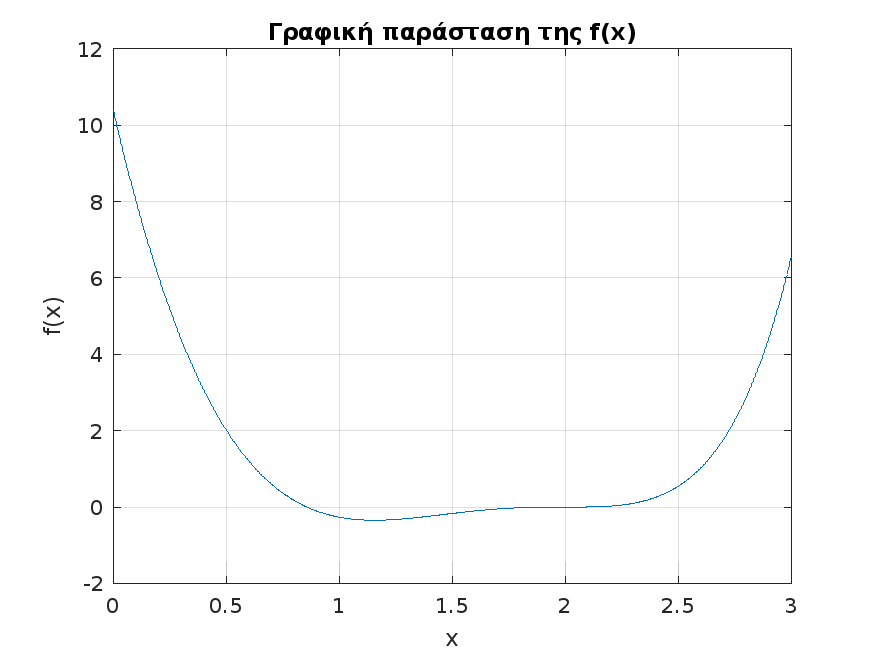
\includegraphics[scale=0.75]{graph1.png}
\end{center}   % End centering.

\subsection*{Α' Ερώτημα - Μέθοδος διχοτόμησης}  % Adds subsection

Γράφτηκε κώδικας της μεθόδου της διχοτόμησης για να προσεγγίσει τις ρίζες της \(f(x) = 14xe^{x-2} - 12e^{x-2} - 7x^3 + 20x^2 - 26x + 12\) στο κλειστό διάστημα \([0,3]\) με ακρίβεια $5$ δεκαδικών ψηφίων (\(\varepsilon = \frac{1}{2} \times 10^5 = 0.000005\)). Προσεγγίζει σωστά και τις δύο ρίζες της \(f\), μια στο σημείο \(m_1 = 0.857142\) με \(N = 19\) επαναλήψεις και μια στο σημείο \(m_2 = 2.000004\) με \(N = 17\) επαναλήψεις. Ο αλγόριθμος για τις συγκεκριμένες ρίζες τρέχει σε σχεδόν μηδενικό χρόνο.\\

Προτού γραφτεί ο κώδικας, ελέγχθηκε αν ισχύει το Θεώρημα Bolzano για το αρχικό διάστημα \([0,3]\). Παρ' όλα αυτά δεν ισχύει γιατί ενώ η \(f\) είναι συνεχής στο \([0,3]\), το \(f(0)\) και το \(f(3)\) είναι ομόσημα, δηλαδή \(f(0) \cdot f(3) > 0\). Άρα ο αλγόριθμος δεν μπορούσε να εφαρμοστεί στο \([0,3]\), οπότε το έσπασα σε δύο διαστήματα, \([0,1.5]\) και \([1.5,3]\) αντίστοιχα. Σε αυτά τα δύο διαστήματα, το Θεώρημα Bolzano ισχύει, εφόσον υπάρχει συνέχεια και η \(f\) είναι ετερόσημη στα άκρα, για κάθε διάστημα.\\

Σχετικά με τον δικό μου κώδικα, υπάρχει μία κύρια συνάρτηση που δέχεται ως είσοδο τα όρια του διαστήματος, \(a\) και \(b\). Έπειτα, ξεκινάει μία επανάληψη \texttt{do-while} που, αρχικά, αυξάνει τον \texttt{loopCounter} κατά ένα και υπολογίζει το μέσο \(m\) του διαστήματος σύμφωνα με τον τύπο \(m = \frac{a+b}{2.0}\). Το μέσο m, αποτελεί την προσέγγιση της ρίζας και ανανεώνεται σε κάθε επανάληψη. Αντί για \(2\), μπήκε \(2.0\) ώστε να επιστραφεί δεκαδικό αποτέλεσμα. Στη συνέχεια, με τη χρήση μιας βοηθητικής συνάρτησης που επιστρέφει την τιμή της \(f\) για κάποιο \(x\), βρίσκω τα \(f(a)\), \(f(b)\), \(f(m)\). Η επανάληψη έχει δύο συνθήκες τερματισμού. Η πρώτη ελέγχει αν η τιμή της \(f(m)\) είναι η μηδενική, άρα το m είναι η ακριβής ρίζα, και αν ισχύει σταματάει. Αν δεν ισχύει, συνεχίζεται ο αλγόριθμος και ανάλογα με το πρόσημο της \(f(a) \cdot f(m)\), δημιουργείται το νέο διάστημα. Συγκεκριμένα, αν \(f(a) \cdot f(m) < 0\) τότε το νέο διάστημα είναι το \([a,m]\), αλλιώς είναι το \([m,b]\). Αυτό γίνεται ώστε να εξακολουθεί να ισχύει το Θεώρημα Bolzano, στο οποίο βασίζεται η μέθοδος της διχοτόμησης. Η δεύτερη συνθήκη, ελέγχει αν η διαφορά \(b-a\) είναι μικρότερη του σφάλαματος, και αν ισχύει σταματάει. Αν δεν ισχύει, ξεκινάει την επανάληψη από την αρχή.\\

Σχετικά με το Chat GPT, το ζήτησα να παράγει έναν παρόμοιο αλγόρθιθμο, δίνοντάς το την εξής είσοδο:
	\begin{quote}
	{\small \emph{Write me a bisection method C code for this function: f(x) = 14 * x * exp(x - 2) - 12 * exp(x - 2) - 7 * x * x * x + 20 * x * x - 26 * x + 12\\
Tolerance of 5 decimal digits.\\
Make it so it runs 2 times, one for interval [0,1.5] and one for interval [1.5,3]. Add loop counter for each of 2 times.}}
	\end{quote}
Ο κώδικας που μου παρήγαγε λειτουργεί, βγάζει τα ίδια αποτελέσματα και αριθμό επαναλήψεων. Οι διαφορές μας είναι στον τρόπο γραφής του αλγορίθμου, όπως σε ονόματα μεταβλητών και διάταξη των if-statements. Επίσης, ο κώδικας του είναι πιο καθαρογραμμένος, αλλα περιέχει λιγότερα σχόλια από τον δικό μου. Οι δύο κώδικες υπάρχουν στον φάκελο \emph{1a}, με ονόματα \emph{`main.c`} και \emph{`chat.gpt`} αντίστοιχα.\\

Τέλος, ο εξής πίνακας περιλαμβάνει χρήσιμες πληροφορίες, οι οποίες αποτελούν και την έξοδο του κάθε κώδικα στην κονσόλα:\\

\vspace{3\baselineskip}

\begin{center}
\setlength{\arraycolsep}{3pt} % Adjust the separation as needed

{\footnotesize
\begin{tabular}{|c|clll|}
\hline
\textbf{Αρχείο} &
  \multicolumn{4}{@{}c@{}|}{\textbf{{[}0, 1.5{]}}} \\ \hline
\multirow{2}{*}{\textbf{main.c}} &
  \multicolumn{1}{@{}c|}{Root Approximation} &
  \multicolumn{1}{@{}l|}{f Value Approximation} &
  \multicolumn{1}{@{}l|}{Loops} &
  Time Approximation \\ \cline{2-5} 
 &
  \multicolumn{1}{@{}l|}{\textit{0.857142}} &
  \multicolumn{1}{@{}l|}{\textit{0.000001}} &
  \multicolumn{1}{@{}l|}{\textit{19}} &
  \textit{0 seconds} \\ \hline
\multicolumn{1}{|l|}{\multirow{2}{*}{\textbf{chatgpt.c}}} &
  \multicolumn{1}{@{}c|}{Root Approximation} &
  \multicolumn{1}{@{}l|}{f Value Approximation} &
  \multicolumn{1}{@{}l|}{Loops} &
  Time Approximation \\ \cline{2-5} 
\multicolumn{1}{|l|}{} &
  \multicolumn{1}{@{}l|}{\textit{0.857142}} &
  \multicolumn{1}{@{}l|}{\textit{0.000001}} &
  \multicolumn{1}{@{}l|}{\textit{19}} &
  \textit{0 seconds} \\ \hline
\end{tabular}
}

\end{center}

\begin{center}
\setlength{\arraycolsep}{3pt} % Adjust the separation as needed

{\footnotesize
\begin{tabular}{|c|clll|}
\hline
\textbf{Αρχείο} &
  \multicolumn{4}{@{}c@{}|}{\textbf{{[}1.5, 3{]}}} \\ \hline
\multirow{2}{*}{\textbf{main.c}} &
  \multicolumn{1}{@{}c|}{Root Approximation} &
  \multicolumn{1}{@{}l|}{f Value Approximation} &
  \multicolumn{1}{@{}l|}{Loops} &
  Time Approximation \\ \cline{2-5} 
 &
  \multicolumn{1}{@{}l|}{\textit{2.000004}} &
  \multicolumn{1}{@{}l|}{\textit{0.000000}} &
  \multicolumn{1}{@{}l|}{\textit{17}} &
  \textit{0 seconds} \\ \hline
\multirow{2}{*}{\textbf{chatgpt.c}} &
  \multicolumn{1}{@{}c|}{Root Approximation} &
  \multicolumn{1}{@{}l|}{f Value Approximation} &
  \multicolumn{1}{@{}l|}{Loops} &
  Time Approximation \\ \cline{2-5} 
 &
  \multicolumn{1}{@{}l|}{\textit{2.000004}} &
  \multicolumn{1}{@{}l|}{\textit{0.000000}} &
  \multicolumn{1}{@{}l|}{\textit{17}} &
  \textit{0 seconds} \\ \hline
\end{tabular}
}

\end{center}

\vspace{2\baselineskip}

\subsection*{Β' Ερώτημα - Μέθοδος Newton-Raphson}  % Adds subsection

Γράφτηκε κώδικας της μεθόδου Newton-Raphson για να προσεγγίσει τις ρίζες της \(f(x) = 14xe^{x-2} - 12e^{x-2} - 7x^3 + 20x^2 - 26x + 12\) στο κλειστό διάστημα \([0,3]\) με ακρίβεια $5$ δεκαδικών ψηφίων (\(\varepsilon = \frac{1}{2} \times 10^5 = 0.000005\)). Για την εκτέλεση του αλγορίθμου, έπρεπε να υπολογιστεί η πρώτη παράγωγος. Έχουμε \(f'(x) = 14xe^{(x-2)} + 2e^{(x-2)} - 21x^2 + 40x - 26\). Προσεγγίζει σωστά και τις δύο ρίζες της \(f\), μια στο σημείο \(m_1 = 0.857143\) με \(N = 7\) επαναλήψεις και μια στο σημείο \(m_2 = 2.000013\) με \(N = 29\) επαναλήψεις. Ο αλγόριθμος για τις συγκεκριμένες ρίζες τρέχει σε σχεδόν μηδενικό χρόνο.\\

Προτού γραφτεί ο κώδικας, διαλέχθηκαν δύο διαστήματα για την εύρεση κάθε ρίζας και ένα αρχικά σημείο για κάθε διάστημα. Το πρώτο διάστημα είναι το \([0,1]\) καθώς η \(f\) είναι δύο φορές παραγωγίσιμη με πρώτη και δεύτερο παράγωγο που δεν μηδενίζονται καθόλου σε αυτό το κλειστό διάστημα, καθώς και ισχύει \(f(0) \cdot f(1)<0\). Έτσι, ικανοποιείται το βασικό θεώρημα στο οποίο βασίζεται η μέθοδος Newton-Raphson. Αρχικό σημείο διαλέχθηκε το \(x_0=0\), καθώς ισχύει \(f(x_0) \cdot f''(x_0) > 0\), το οποίο είναι απαραίτητο για τον αλγόριθμο. Με παρόμοια λογική, για την εύρεση της δεύτερης ρίζας διαλέχθηκε το \([2,3]\) με \(x_0=3\). (Για την ακρίβεια, κοντά στο 2, η πρώτη αλλά και η δεύτερη παράγωγος μηδενίζεται. Η επίπτωση που έχει αυτό θα αναλυθεί παρακάτω.)\\

Σχετικά με τον δικό μου κώδικα, υπάρχει μία κύρια συνάρτηση με είσοδο την αρχική τιμή \(x_0\) της αναδρομικής ακολουθίας προσέγγισης ριζών. Έπειτα, ξεκινάει μία επανάληψη \texttt{do-while} που, αρχικά, αυξάνει τον \texttt{loopCounter} κατά ένα και βρίσκει την επόμενη προσέγγιση ρίζας σύμφωνα με τον τύπο \(x_{n+1} = x_n - \frac{f(x_n)}{f'(x_n)}\). Για την εκτέλεση αυτής της εντολής, έχουν προγραμματιστεί κατάλληλες συναρτήσεις που επιστρέφουν την τιμή της \(f(x)\) και \(f'(x)\) αντίστοιχα. Η επανάληψη σταματάει όταν ισχύσει \(f(x_{n}) = 0.0\) \textbf{ή} \(|x_{n-1} - x_n| < \varepsilon\), oι οποίες σχέσεις αποτελούν τις βασικές συνθήκες τερματισμού της μεθόδου Newton-Raphson.\\

Σχετικά με το Chat GPT, το ζήτησα να παράγει έναν παρόμοιο αλγόρθιθμο, δίνοντάς το την εξής είσοδο:
	\begin{quote}
	{\small \emph{Write me a Newton-Raphson method C code for this function: f(x) = 14 * x * exp(x - 2) - 12 * exp(x - 2) - 7 * x * x * x + 20 * x * x - 26 * x + 12
Tolerance of 5 decimal digits.
Make it so it runs 2 times, one for x0=0 and one for x0=3. Add loop counter for each of 2 times.}}
	\end{quote}
Ο κώδικας που μου παρήγαγε είχε λογικό λάθος στη συνάρτηση της παραγώγου, οπότε έπρεπε να το διορθώσω. Ο πλέον διορθωμένος κώδικας του Chat GPT βγάζει τα ίδια αποτελέσματα και αριθμό επαναλήψεων. Οι διαφορές μας είναι στον τρόπο γραφής του αλγορίθμου, όπως σε ονόματα μεταβλητών. Επίσης, ο κώδικας περιέχει λιγότερα σχόλια από τον δικό μου. Οι δύο κώδικες υπάρχουν στον φάκελο \emph{1b}, με ονόματα \emph{`main.c`} και \emph{`chat.gpt`} αντίστοιχα.\\

Τέλος, ο εξής πίνακας περιλαμβάνει χρήσιμες πληροφορίες, οι οποίες αποτελούν και την έξοδο του κάθε κώδικα στην κονσόλα:\\

\begin{center}
\setlength{\arraycolsep}{3pt} % Adjust the separation as needed

{\footnotesize
\begin{tabular}{|c|clll|}
\hline
\textbf{Αρχείο} &
  \multicolumn{4}{@{}c@{}|}{\(x_0=0\)} \\ \hline
\multirow{2}{*}{\textbf{main.c}} &
  \multicolumn{1}{@{}c|}{Root Approximation} &
  \multicolumn{1}{@{}l|}{f Value Approximation} &
  \multicolumn{1}{@{}l|}{Loops} &
  Time Approximation \\ \cline{2-5} 
 &
  \multicolumn{1}{@{}l|}{\textit{0.857143}} &
  \multicolumn{1}{@{}l|}{\textit{0.000000}} &
  \multicolumn{1}{@{}l|}{\textit{7}} &
  \textit{0 seconds} \\ \hline
\multicolumn{1}{|l|}{\multirow{2}{*}{\textbf{chatgpt.c}}} &
  \multicolumn{1}{@{}c|}{Root Approximation} &
  \multicolumn{1}{@{}l|}{f Value Approximation} &
  \multicolumn{1}{@{}l|}{Loops} &
  Time Approximation \\ \cline{2-5} 
\multicolumn{1}{|l|}{} &
  \multicolumn{1}{@{}l|}{\textit{0.857143}} &
  \multicolumn{1}{@{}l|}{\textit{0.000000}} &
  \multicolumn{1}{@{}l|}{\textit{7}} &
  \textit{0 seconds} \\ \hline
\end{tabular}
}

\end{center}

\begin{center}
\setlength{\arraycolsep}{3pt} % Adjust the separation as needed

{\footnotesize
\begin{tabular}{|c|clll|}
\hline
\textbf{Αρχείο} &
  \multicolumn{4}{@{}c@{}|}{\(x_0=3\)} \\ \hline
\multirow{2}{*}{\textbf{main.c}} &
  \multicolumn{1}{@{}c|}{Root Approximation} &
  \multicolumn{1}{@{}l|}{f Value Approximation} &
  \multicolumn{1}{@{}l|}{Loops} &
  Time Approximation \\ \cline{2-5} 
 &
  \multicolumn{1}{@{}l|}{\textit{2.000013}} &
  \multicolumn{1}{@{}l|}{\textit{0.000000}} &
  \multicolumn{1}{@{}l|}{\textit{29}} &
  \textit{0 seconds} \\ \hline
\multirow{2}{*}{\textbf{chatgpt.c}} &
  \multicolumn{1}{@{}c|}{Root Approximation} &
  \multicolumn{1}{@{}l|}{f Value Approximation} &
  \multicolumn{1}{@{}l|}{Loops} &
  Time Approximation \\ \cline{2-5} 
 &
  \multicolumn{1}{@{}l|}{\textit{2.000013}} &
  \multicolumn{1}{@{}l|}{\textit{0.000000}} &
  \multicolumn{1}{@{}l|}{\textit{29}} &
  \textit{0 seconds} \\ \hline
\end{tabular}
}

\end{center}

Σχετικά με τη σύγκλιση, ας μελετήσουμε τις δύο ακολουθίες προσέγγισης ρίζας.
Για \(x_0=0\), η πορεία προσεγγίσεων είναι η εξής:
\begin{quote}
	{\small \emph{0.000000\\0.403274\\0.660722\\0.801056\\0.850752\\0.857046\\0.857143}}
\end{quote}
Για \(x_0=3\), η πορεία προσεγγίσεων είναι η εξής:
\begin{quote}
	{\small \emph{3.000000\\2.733850\\2.529772\\2.376666\\2.264146\\2.183031\\2.125566\\2.085462\\2.057815\\2.038938\\2.026141\\2.017511\\2.011711\\2.007825\\2.005224\\2.003486\\2.002326
	\\2.001551\\2.001034\\2.000690\\2.000460\\2.000307\\2.000204\\2.000136\\2.000091\\2.000060\\2.000040\\2.000026\\2.000016}}
\end{quote}
Εύκολα βλέπουμε ότι για την εύρεση της πρώτης ρίζας με \(x_0=0\), η μέθοδος Newton-Raphson συγκλίνει τετραγωνικά (το τετράγωνο της επόμενης τιμής της ακολουθίας είναι κοντά στην προηγούμενη τιμή).
Αυτό όμως δεν ισχυέι για την εύρεση της δεύτερης ρίζας με \(x_0=3\). Αρχικά, και οι δύο αρχικές προσεγγίσεις είναι κοντά στην ρίζα, οπότε δεν επηρεάζει σημαντικά τη σύγκλιση. Η αιτία που τη δεύτερη φορά η μέθοδος δε συγκλίνει τετραγωνικά είναι το γεγονός ότι η πρώτη και η δεύτερη παράγωγος μηδενίζονται κοντά στη ρίζα της συνάρτησης.

\vspace{2\baselineskip}

\subsection*{Γ' Ερώτημα - Μέθοδος Τέμνουσας}  % Adds subsection

Γράφτηκε κώδικας της μεθόδους της τέμνουσας για να προσεγγίσει τις ρίζες της \(f(x) = 14xe^{x-2} - 12e^{x-2} - 7x^3 + 20x^2 - 26x + 12\) στο κλειστό διάστημα \([0,3]\) με ακρίβεια $5$ δεκαδικών ψηφίων (\(\varepsilon = \frac{1}{2} \times 10^5 = 0.000005\)). Προσεγγίζει σωστά και τις δύο ρίζες της \(f\), μια στο σημείο \(m_1 = 0.857143\) με \(N = 8\) επαναλήψεις και μια στο σημείο \(m_2 = 1.999990\) με \(N = 35\) επαναλήψεις. Ο αλγόριθμος για τις συγκεκριμένες ρίζες τρέχει σε σχεδόν μηδενικό χρόνο.\\

Προτού γραφτεί ο κώδικας, διαλέχθηκαν δύο διαστήματα για την εύρεση κάθε ρίζας και δύο αρχικά σημεία για κάθε διάστημα. Το πρώτο διάστημα είναι το \([0,1]\) καθώς η \(f\) είναι δύο φορές παραγωγίσιμη με πρώτη και δεύτερο παράγωγο που δεν μηδενίζονται καθόλου σε αυτό το κλειστό διάστημα, καθώς και ισχύει \(f(0) \cdot f(1)<0\). Έτσι, ικανοποιείται το βασικό θεώρημα στο οποίο βασίζεται η μέθοδος της τέμνουσας. Αρχικά σημεία διαλέχθηκαν τα άκρα του διαστήματος, δηλαδή το \(x_0=0\) και το \(x_1=1\). Με παρόμοια λογική, για την εύρεση της δεύτερης ρίζας διαλέχθηκε \(x_0=1.5\) και \(x_1=1.7\). \\

Σχετικά με τον δικό μου κώδικα, υπάρχει μία κύρια συνάρτηση με είσοδο τις αρχικές τιμές \(x_0\) και \(x_1\) της αναδρομικής ακολουθίας προσέγγισης ριζών. Έπειτα, ξεκινάει μία επανάληψη \texttt{do-while} που, αρχικά, αυξάνει τον \texttt{loopCounter} και αμέσως μετά ελέγχει αν ένα από τα \(x_{n-1}\) ή \(x_n\) είναι μηδέν, ώστε να σταματήσει εφόσον βρει τη ρίζα. Έπειτα, υπολογίζει το \(x_{n+1}\) από τον τύπο: \(x_{n+1} = x_n - \frac{f(x_n) \cdot (x_n - x_{n-1})}{f(x_n) - f(x_{n-1})}\). Τέλος, ελέγχει αν \(|x_{n-1} - x_n| < \varepsilon\), ώστε να σταματήσει λόγω του σφάλματος που θέσαμε.\\

Σχετικά με το Chat GPT, το ζήτησα να παράγει έναν παρόμοιο αλγόρθιθμο, δίνοντάς το την εξής είσοδο:
	\begin{quote}
	{\small \emph{Write me a secant method C code for this function: f(x) = 14 * x * exp(x - 2) - 12 * exp(x - 2) - 7 * x * x * x + 20 * x * x - 26 * x + 12
Tolerance of 5 decimal digits.
Make it so it runs 2 times, one for interval x0=0 and x1=1 and one for interval x0=1.5 and x1=1.7. Add loop counter for each of 2 times.}}
	\end{quote}
Ο κώδικας που μου παρήγαγε λειτουργεί, οι ρίζες του προσεγγίζουν τους ίδιους αριθμούς με εμένα αλλά είναι λίγο διαφορετικές. Στη δεύτερη ρίζα, σταματάει νωρίτερα βρίσκοντας μακρινότερη προσέγγιση. Επίσης, ο κώδικάς του περιέχει λιγότερα σχόλια από τον δικό μου. Οι δύο κώδικες υπάρχουν στον φάκελο \emph{1c}, με ονόματα \emph{`main.c`} και \emph{`chat.gpt`} αντίστοιχα.\\

Τέλος, ο εξής πίνακας περιλαμβάνει χρήσιμες πληροφορίες, οι οποίες αποτελούν και την έξοδο του κάθε κώδικα στην κονσόλα:\\

\begin{center}
\setlength{\arraycolsep}{3pt} % Adjust the separation as needed

{\footnotesize
\begin{tabular}{|c|clll|}
\hline
\textbf{Αρχείο} &
  \multicolumn{4}{@{}c@{}|}{\(x_0=0\), \(x_1=1\)} \\ \hline
\multirow{2}{*}{\textbf{main.c}} &
  \multicolumn{1}{@{}c|}{Root Approximation} &
  \multicolumn{1}{@{}l|}{f Value Approximation} &
  \multicolumn{1}{@{}l|}{Loops} &
  Time Approximation \\ \cline{2-5} 
 &
  \multicolumn{1}{@{}l|}{\textit{0.857143}} &
  \multicolumn{1}{@{}l|}{\textit{0.000000}} &
  \multicolumn{1}{@{}l|}{\textit{8}} &
  \textit{0 seconds} \\ \hline
\multicolumn{1}{|l|}{\multirow{2}{*}{\textbf{chatgpt.c}}} &
  \multicolumn{1}{@{}c|}{Root Approximation} &
  \multicolumn{1}{@{}l|}{f Value Approximation} &
  \multicolumn{1}{@{}l|}{Loops} &
  Time Approximation \\ \cline{2-5} 
\multicolumn{1}{|l|}{} &
  \multicolumn{1}{@{}l|}{\textit{0.857143}} &
  \multicolumn{1}{@{}l|}{\textit{-0.000000}} &
  \multicolumn{1}{@{}l|}{\textit{7}} &
  \textit{0 seconds} \\ \hline
\end{tabular}
}

\end{center}

\begin{center}
\setlength{\arraycolsep}{3pt} % Adjust the separation as needed

{\footnotesize
\begin{tabular}{|c|clll|}
\hline
\textbf{Αρχείο} &
  \multicolumn{4}{@{}c@{}|}{\(x_0=1.5\), \(x_1=1.7\)} \\ \hline
\multirow{2}{*}{\textbf{main.c}} &
  \multicolumn{1}{@{}c|}{Root Approximation} &
  \multicolumn{1}{@{}l|}{f Value Approximation} &
  \multicolumn{1}{@{}l|}{Loops} &
  Time Approximation \\ \cline{2-5} 
 &
  \multicolumn{1}{@{}l|}{\textit{1.999990}} &
  \multicolumn{1}{@{}l|}{\textit{0.000000}} &
  \multicolumn{1}{@{}l|}{\textit{35}} &
  \textit{0 seconds} \\ \hline
\multirow{2}{*}{\textbf{chatgpt.c}} &
  \multicolumn{1}{@{}c|}{Root Approximation} &
  \multicolumn{1}{@{}l|}{f Value Approximation} &
  \multicolumn{1}{@{}l|}{Loops} &
  Time Approximation \\ \cline{2-5} 
 &
  \multicolumn{1}{@{}l|}{\textit{1.991455}} &
  \multicolumn{1}{@{}l|}{\textit{-0.000002}} &
  \multicolumn{1}{@{}l|}{\textit{12}} &
  \textit{0 seconds} \\ \hline
\end{tabular}
}

\end{center}

\vspace{2\baselineskip}

\section*{Δεύτερη Άσκηση}   % Starts second exercise

\subsection*{Γενικά σχόλια για τους κώδικες της άσκησης}   % Adds subsection
	Για την συγκεκριμένη άσκηση, όπως και για την προηγούμενη, \textbf{δεν χρησιμοποιήθηκε καθόλου κάποιο γλωσσικό μοντέλο για την διευκόλυνση της γραφής του δικού μου κώδικα.} Παρ'όλα αυτά, αφού έλυσα κάθε υποερώτημα, έδωσα την εκφώνησή του στο ChatGPT, για να μου παρουσιάσει και τη δικιά του λύση, την οποία παραθέτω και συγκρίνω με τη δικιά μου σε κάθε υποερώτημα. Οι καθαρά δικοί μου κώδικες έχουν όνομα \emph{`main.c`} και οι κώδικες του ChatGPT έχουν όνομα \emph{`chatgpt.c`}, σε μερικούς από τους οποίους χρειάστηκε να παρέμβω, προσθέτοντας βοηθητικές εξόδους, κώδικες για καταγραφή χρόνου εκτέλεσης, κλπ. Σε ό,τι αλλαγεί έχω κάνει εγώ σε κώδικα του Chat GPT άφησα ένα σχόλιο από δίπλα (\texttt{//I added this}). Αναλυτικότερες λεπτομέρειες θα αναφερθούν σε κάθε υποερώτημα.

\subsection*{Α' Ερώτημα - Τροποποιημένη μέθοδος Newton-Raphson}   % Adds subsection

Γράφτηκε κώδικας μιας τροποιημένης μεθόδου Newton-Raphson για να προσεγγίσει τις ρίζες της \(f(x) = 54x^6 + 45x^5 - 102x^4 - 69x^3 + 35x^2 + 16x - 4\) στο κλειστό διάστημα \([-2,2]\) με ακρίβεια $5$ δεκαδικών ψηφίων (\(\varepsilon = \frac{1}{2} \times 10^5 = 0.000005\)). Για την εκτέλεση του αλγορίθμου, έπρεπε να υπολογιστούν η πρώτη και δεύτερη παράγωγος. Έχουμε \(f'(x) = 324x^5 + 225x^4 - 408x^3 - 207x^2 + 70x + 16\) και \(f''(x) = 1620x^4 + 900x^3 - 1224x^2 - 414x + 70\). Προσεγγίζει σωστά και τις πέντε ρίζες της \(f\), μια στο σημείο \(m_1 = -1.381298\) με \(N = 5\) επαναλήψεις, μια στο σημείο \(m_2 = -0.666668\) με \(N = 12\) επαναλήψεις, μια στο σημείο \(m_3 = 0.205183\) με \(N = 4\) επαναλήψεις, μια στο σημείο \(m_4 = 0.500000\) με \(N = 4\) επαναλήψεις και μια στο σημείο \(m_5 = 1.176116\) με \(N = 5\) επαναλήψεις. Ο αλγόριθμος για τις συγκεκριμένες ρίζες τρέχει σε σχεδόν μηδενικό χρόνο.\\

Προτού γραφτεί ο κώδικας, διαλέχθηκαν τα εξής αρχικά σημεία: -2, -1, 0, 0.4, 1 με παρόμοια λογική με την απλή μέθοδο. Δηλαδή, για κάθε ένα από αυτά ισχύει \(f(x)*f''(x)>0\).\\

Σχετικά με τον δικό μου κώδικα, υπάρχει μία κύρια συνάρτηση με είσοδο την αρχική τιμή \(x_0\) της αναδρομικής ακολουθίας προσέγγισης ριζών. Έπειτα, ξεκινάει μία επανάληψη \texttt{do-while} που, αρχικά, αυξάνει τον \texttt{loopCounter} κατά ένα και βρίσκει την επόμενη προσέγγιση ρίζας σύμφωνα με τον τροποποιημένου τύπο \(x_{n+1} = x_n - \frac{f(x_n)}{\frac{f'(x_n)}{f(x_n)} - \frac{1}{2} \frac{f''(x_n)}{f'(x_n)}}\). Για την εκτέλεση αυτής της εντολής, έχουν προγραμματιστεί κατάλληλες συναρτήσεις που επιστρέφουν την τιμή της \(f(x)\), της \(f'(x)\) και \(f''(x)\) της αντίστοιχα. Η επανάληψη σταματάει όταν ισχύσει \(f(x_{n}) = 0.0\) \textbf{ή} \(|x_{n-1} - x_n| < \varepsilon\), oι οποίες σχέσεις αποτελούν τις βασικές συνθήκες τερματισμού της μεθόδου Newton-Raphson.\\

Σχετικά με το Chat GPT, το ζήτησα να παράγει έναν παρόμοιο αλγόρθιθμο, δίνοντάς το την εξής είσοδο:
	\begin{quote}
	{\small \emph{Write me a Newton-Raphson method C code for this function: f(x) = 54 * x * x * x * x * x * x + 45 * x * x * x * x * x - 102 * x * x * x * x - 69 * x * x * x + 35 * x * x + 16 * x - 4
Tolerance of 5 decimal digits.
Make it so it runs 5 times, one for n0=-2, n0=-1, n0=0, n0=0.4, n0=1.
New approximation point = x - (1 / ( f`(x)/f(x) - 0.5*f``(x)/f`(x) ) )}}
	\end{quote}
Ο κώδικας που μου παρήγαγε είχε λογικό λάθος στη συνάρτηση της πρώτης και δεύτερης παραγώγου, οπότε έπρεπε να το διορθώσω. Ο πλέον διορθωμένος κώδικας του Chat GPT βγάζει τα ίδια αποτελέσματα και αριθμό επαναλήψεων. Οι διαφορές μας είναι στον τρόπο γραφής του αλγορίθμου, όπως σε ονόματα μεταβλητών. Επίσης, ο κώδικας περιέχει λιγότερα σχόλια από τον δικό μου. Οι δύο κώδικες υπάρχουν στον φάκελο \emph{2a}, με ονόματα \emph{`main.c`} και \emph{`chat.gpt`} αντίστοιχα.\\

Τέλος, ο εξής πίνακας περιλαμβάνει χρήσιμες πληροφορίες, οι οποίες αποτελούν και την έξοδο του κάθε κώδικα στην κονσόλα:\\

\begin{center}
\setlength{\arraycolsep}{3pt} % Adjust the separation as needed

{\footnotesize
\begin{tabular}{|c|clll|}
\hline
\textbf{Αρχείο} &
  \multicolumn{4}{@{}c@{}|}{\(x_0=-2\)} \\ \hline
\multirow{2}{*}{\textbf{main.c}} &
  \multicolumn{1}{@{}c|}{Root Approximation} &
  \multicolumn{1}{@{}l|}{f Value Approximation} &
  \multicolumn{1}{@{}l|}{Loops} &
  Time Approximation \\ \cline{2-5} 
 &
  \multicolumn{1}{@{}l|}{\textit{-1.381298}} &
  \multicolumn{1}{@{}l|}{\textit{-0.000000}} &
  \multicolumn{1}{@{}l|}{\textit{5}} &
  \textit{0 seconds} \\ \hline
\multicolumn{1}{|l|}{\multirow{2}{*}{\textbf{chatgpt.c}}} &
  \multicolumn{1}{@{}c|}{Root Approximation} &
  \multicolumn{1}{@{}l|}{f Value Approximation} &
  \multicolumn{1}{@{}l|}{Loops} &
  Time Approximation \\ \cline{2-5} 
\multicolumn{1}{|l|}{} &
  \multicolumn{1}{@{}l|}{\textit{-1.381298}} &
  \multicolumn{1}{@{}l|}{\textit{-0.000000}} &
  \multicolumn{1}{@{}l|}{\textit{5}} &
  \textit{0 seconds} \\ \hline
\end{tabular}
}

\end{center}

\begin{center}
\setlength{\arraycolsep}{3pt} % Adjust the separation as needed

{\footnotesize
\begin{tabular}{|c|clll|}
\hline
\textbf{Αρχείο} &
  \multicolumn{4}{@{}c@{}|}{\(x_0=-1\)} \\ \hline
\multirow{2}{*}{\textbf{main.c}} &
  \multicolumn{1}{@{}c|}{Root Approximation} &
  \multicolumn{1}{@{}l|}{f Value Approximation} &
  \multicolumn{1}{@{}l|}{Loops} &
  Time Approximation \\ \cline{2-5} 
 &
  \multicolumn{1}{@{}l|}{\textit{-0.666668}} &
  \multicolumn{1}{@{}l|}{\textit{-0.000000}} &
  \multicolumn{1}{@{}l|}{\textit{12}} &
  \textit{0 seconds} \\ \hline
\multirow{2}{*}{\textbf{chatgpt.c}} &
  \multicolumn{1}{@{}c|}{Root Approximation} &
  \multicolumn{1}{@{}l|}{f Value Approximation} &
  \multicolumn{1}{@{}l|}{Loops} &
  Time Approximation \\ \cline{2-5} 
 &
  \multicolumn{1}{@{}l|}{\textit{-0.666668}} &
  \multicolumn{1}{@{}l|}{\textit{-0.000000}} &
  \multicolumn{1}{@{}l|}{\textit{12}} &
  \textit{0 seconds} \\ \hline
\end{tabular}
}

\end{center}

\begin{center}
\setlength{\arraycolsep}{3pt} % Adjust the separation as needed

{\footnotesize
\begin{tabular}{|c|clll|}
\hline
\textbf{Αρχείο} &
  \multicolumn{4}{@{}c@{}|}{\(x_0=0\)} \\ \hline
\multirow{2}{*}{\textbf{main.c}} &
  \multicolumn{1}{@{}c|}{Root Approximation} &
  \multicolumn{1}{@{}l|}{f Value Approximation} &
  \multicolumn{1}{@{}l|}{Loops} &
  Time Approximation \\ \cline{2-5} 
 &
  \multicolumn{1}{@{}l|}{\textit{0.205183}} &
  \multicolumn{1}{@{}l|}{\textit{-0.000000}} &
  \multicolumn{1}{@{}l|}{\textit{4}} &
  \textit{0 seconds} \\ \hline
\multirow{2}{*}{\textbf{chatgpt.c}} &
  \multicolumn{1}{@{}c|}{Root Approximation} &
  \multicolumn{1}{@{}l|}{f Value Approximation} &
  \multicolumn{1}{@{}l|}{Loops} &
  Time Approximation \\ \cline{2-5} 
 &
  \multicolumn{1}{@{}l|}{\textit{0.205183}} &
  \multicolumn{1}{@{}l|}{\textit{0.000000}} &
  \multicolumn{1}{@{}l|}{\textit{4}} &
  \textit{0 seconds} \\ \hline
\end{tabular}
}

\end{center}

\begin{center}
\setlength{\arraycolsep}{3pt} % Adjust the separation as needed

{\footnotesize
\begin{tabular}{|c|clll|}
\hline
\textbf{Αρχείο} &
  \multicolumn{4}{@{}c@{}|}{\(x_0=0.4\)} \\ \hline
\multirow{2}{*}{\textbf{main.c}} &
  \multicolumn{1}{@{}c|}{Root Approximation} &
  \multicolumn{1}{@{}l|}{f Value Approximation} &
  \multicolumn{1}{@{}l|}{Loops} &
  Time Approximation \\ \cline{2-5} 
 &
  \multicolumn{1}{@{}l|}{\textit{0.500000}} &
  \multicolumn{1}{@{}l|}{\textit{0.000000}} &
  \multicolumn{1}{@{}l|}{\textit{4}} &
  \textit{0 seconds} \\ \hline
\multirow{2}{*}{\textbf{chatgpt.c}} &
  \multicolumn{1}{@{}c|}{Root Approximation} &
  \multicolumn{1}{@{}l|}{f Value Approximation} &
  \multicolumn{1}{@{}l|}{Loops} &
  Time Approximation \\ \cline{2-5} 
 &
  \multicolumn{1}{@{}l|}{\textit{0.500000}} &
  \multicolumn{1}{@{}l|}{\textit{0.000000}} &
  \multicolumn{1}{@{}l|}{\textit{4}} &
  \textit{0 seconds} \\ \hline
\end{tabular}
}

\end{center}

\begin{center}
\setlength{\arraycolsep}{3pt} % Adjust the separation as needed

{\footnotesize
\begin{tabular}{|c|clll|}
\hline
\textbf{Αρχείο} &
  \multicolumn{4}{@{}c@{}|}{\(x_0=1\)} \\ \hline
\multirow{2}{*}{\textbf{main.c}} &
  \multicolumn{1}{@{}c|}{Root Approximation} &
  \multicolumn{1}{@{}l|}{f Value Approximation} &
  \multicolumn{1}{@{}l|}{Loops} &
  Time Approximation \\ \cline{2-5} 
 &
  \multicolumn{1}{@{}l|}{\textit{1.176116}} &
  \multicolumn{1}{@{}l|}{\textit{-0.000000}} &
  \multicolumn{1}{@{}l|}{\textit{5}} &
  \textit{0 seconds} \\ \hline
\multirow{2}{*}{\textbf{chatgpt.c}} &
  \multicolumn{1}{@{}c|}{Root Approximation} &
  \multicolumn{1}{@{}l|}{f Value Approximation} &
  \multicolumn{1}{@{}l|}{Loops} &
  Time Approximation \\ \cline{2-5} 
 &
  \multicolumn{1}{@{}l|}{\textit{1.176116}} &
  \multicolumn{1}{@{}l|}{\textit{0.000000}} &
  \multicolumn{1}{@{}l|}{\textit{5}} &
  \textit{0 seconds} \\ \hline
\end{tabular}
}

\end{center}

\subsection*{Α' Ερώτημα - Τροποποιημένη μέθοδος διχοτόμησης}   % Adds subsection

Γράφτηκε κώδικας μιας τροποιημένης μεθόδου διχοτόμησης για να προσεγγίσει τις ρίζες της \(f(x) = 54x^6 + 45x^5 - 102x^4 - 69x^3 + 35x^2 + 16x - 4\) στο κλειστό διάστημα \([-2,2]\) με ακρίβεια $5$ δεκαδικών ψηφίων (\(\varepsilon = \frac{1}{2} \times 10^5 = 0.000005\)). Προσεγγίζει σωστά και τις πέντε ρίζες της \(f\). Σε κάθε εκτέλεση, λόγω της τυχαίας επιλογής, οι προσεγγίσεις είναι λίγο διαφορετικές με πολύ μικρή διαφορά. Οι προσεγγίσεις είναι παρόμοιες με αυτές στην τροποποιημένη Newton-Raphson. Επίσης, η εύρεση της δεύτερης ρίζας αποτελεί μια ειδική περίπτωση, η οποία θα αναλυθεί παρακάτω.\\

Το αρχικό διάστημα, έσπασε στα εξής: \([-2,-1]\), \([-1,0]\), \([0,0.4]\), \([0.4,1]\), \([1,1.2]\), επειδή στα 4 από αυτά ισχύει το θεώρημα Bolzano, στο οποίο βασίζεται η μέθοδος διχοτόμησης. Στο δέυτερο διάστημα \([-1,0]\) το θεώρημα Bolzano δεν ισχύει. Η επίπτωση αυτού του φαινομένου θα αναλυθεί παρακάτω.\\

Σχετικά με τον δικό μου κώδικα, υπάρχει μία κύρια συνάρτηση που δέχεται ως είσοδο τα όρια του διαστήματος, \(a\) και \(b\). Έπειτα, ξεκινάει μία επανάληψη \texttt{do-while} που, αρχικά, αυξάνει τον \texttt{loopCounter} κατά ένα και υπολογίζει την νέα προσέγγιση \(m\) του διαστήματος σύμφωνα με τον τροποιημένο τύπο \texttt{r = ((double)rand() / RANDMAX) * (b - a) + a;} ο οποίος παράγει μια τυχαία τιμή μεταξύ του διαστήματος. Στη συνέχεια, με τη χρήση μιας βοηθητικής συνάρτησης που επιστρέφει την τιμή της \(f\) για κάποιο \(x\), βρίσκω τα \(f(a)\), \(f(b)\), \(f(m)\). Η επανάληψη έχει δύο συνθήκες τερματισμού. Η πρώτη ελέγχει αν \(f(m) < ε\), άρα το m είναι καλή προσσέγιση της ρίζας, και αν ισχύει σταματάει. Αν δεν ισχύει, συνεχίζεται ο αλγόριθμος και ανάλογα με το πρόσημο της \(f(a) \cdot f(m)\), δημιουργείται το νέο διάστημα. Συγκεκριμένα, αν \(f(a) \cdot f(m) < 0\) τότε το νέο διάστημα είναι το \([a,m]\), αλλιώς αν \(f(b) \cdot f(m) < 0\) είναι το \([m,b]\). Αυτό γίνεται ώστε να εξακολουθεί να ισχύει το Θεώρημα Bolzano, όποτε είναι δυνατό, στο οποίο βασίζεται η μέθοδος της διχοτόμησης. Η δεύτερη συνθήκη, ελέγχει αν η διαφορά \(b-a\) είναι μικρότερη του σφάλαματος, και αν ισχύει σταματάει. Αν δεν ισχύει, ξεκινάει την επανάληψη από την αρχή.\\

Σχετικά με το Chat GPT, το ζήτησα να παράγει έναν παρόμοιο αλγόρθιθμο, δίνοντάς το την εξής είσοδο:
	\begin{quote}
	{\small \emph{Write me a bisection method C code for this function: f(x) = 54 * x * x * x * x * x * x + 45 * x * x * x * x * x - 102 * x * x * x * x - 69 * x * x * x + 35 * x * x + 16 * x - 4
Tolerance of 5 decimal digits.
Make it so it runs 5 times, one for interval [-2,-1], one for interval [-1,0], one for interval [0,0.4], one for [0.4, 1] and one for [1,1.2]. Add loop counter for each of 5 times.
Make it so the root approximation each time is not the median, but a random variable between a and b, borders of interval.}}
	\end{quote}
Ο κώδικας που μου παρήγαγε λειτουργεί, βγάζει παρόμοιες ρίζες με παρόμοιο αριθμό επαναλήψεων, εκτός από το δεύτερο διάστημα \([-1,0]\). Σε αυτό το διάστημα, παρ'όλο που ο δικός μου κώδικας είναι σωστός, ο δικός του παράγει μια τελείως λανθασμένη προσέγγιση. Αυτό συμβαίνει γιατί υπάρχει λογικό λάθος στο εξής σημείο του κώδικα του Chat GPT:
	\begin{quote}
	{\small \texttt{if (fa * fc < 0)\\
           b = c;\\
        else\\
           a = c;\\
      }}
	\end{quote}
Όπως αναφέρθηκε πάνω, στο δεύτερο διάστημα το θεώρημα Bolzano δεν ισχύει, οπότε αν δεν ισχύει \texttt{(fa * fc < 0)} δεν σημαίνει ότι απαραίτητα θα ισχύει ότι \texttt{(fb * fc < 0)}. Δηλαδή, εφόσον δεν ισχύει το Bolzano, η f στα άκρα δεν είναι ετερόσημη, άρα τα \texttt{fa, fb, fc} είναι ομόσημα, και στη συγκεκριμένη συνάρτηση αρνητικά. Επομένως, γίνεται η ανάθεση \texttt{a = c;} χωρίς να πρέπει. Έτσι, αλλοιώνεται το διάστημα και παράγεται λογικό λάθος. Η σωστή εκδοχή, βρίσκεται στον δικό μου κώδικα:
	\begin{quote}
	{\small \texttt{if (fa * fr < 0)\\
        b = r;\\
      else if (fb * fr < 0)\\
        a = r;\\
     }}
	\end{quote}
Εδώ, ελέγχω αν ισχύει και \texttt{(fb * fr < 0)} πρωτού γίνει η ανάθεση. Για το δεύτερο διάστημα, στο οποίο δεν ισχύει το Bolzano, δεν θα μπει σε κανένα από τα δύο blocks, με αποτέλεσμα το διάστημα να μένει σταθερό και η εύρεση μιας προσέγγισης να βασίζεται καθαρά στην τύχη, δηλαδή στην ανάθεση μιας τυχαίας  τιμής από την rand. Γι'αυτό τον λόγο, χρειάζονται πολύ περισσότερες επαναλήψεις από τα άλλα διαστήματα. Εκτός από αυτό, υπάρχουν και άλλες διαφορές, όπως στον τρόπο γραφής του αλγορίθμου, σε ονόματα μεταβλητών και διάταξη των if-statements. Επίσης, ο κώδικας του είναι πιο καθαρογραμμένος, αλλα περιέχει λιγότερα σχόλια από τον δικό μου. Οι δύο κώδικες υπάρχουν στον φάκελο \emph{2b}, με ονόματα \emph{`main.c`} και \emph{`chat.gpt`} αντίστοιχα.\\

Τέλος, ο εξής πίνακας περιλαμβάνει χρήσιμες πληροφορίες, οι οποίες αποτελούν και την έξοδο του κάθε κώδικα στην κονσόλα \textbf{για κάποια εκτέλεση}, αφού λόγω της rand, θα υπάρχουν διαφορές στις εκτελέσεις. Οι διαφορές αυτές είναι πολύ μικρές, εκτός από αυτήν που αφορά τον αριθμό επαναλήψεων του αλγορίθμου για το δεύτερο διάστημα. η οποία μπορεί να είναι εκατοντάδες ή και χιλιάδες επαναλήψεις σε κάθε εκτέλεση, επειδή η εύρεση μιας προσέγγισης εξαρτάται καθαρά από την τύχη:\\

\begin{center}
\setlength{\arraycolsep}{3pt} % Adjust the separation as needed

{\footnotesize
\begin{tabular}{|c|clll|}
\hline
\textbf{Αρχείο} &
  \multicolumn{4}{@{}c@{}|}{\([-2,-1]\)} \\ \hline
\multirow{2}{*}{\textbf{main.c}} &
  \multicolumn{1}{@{}c|}{Root Approximation} &
  \multicolumn{1}{@{}l|}{f Value Approximation} &
  \multicolumn{1}{@{}l|}{Loops} &
  Time Approximation \\ \cline{2-5} 
 &
  \multicolumn{1}{@{}l|}{\textit{-1.381303}} &
  \multicolumn{1}{@{}l|}{\textit{0.000968}} &
  \multicolumn{1}{@{}l|}{\textit{22}} &
  \textit{0 seconds} \\ \hline
\multicolumn{1}{|l|}{\multirow{2}{*}{\textbf{chatgpt.c}}} &
  \multicolumn{1}{@{}c|}{Root Approximation} &
  \multicolumn{1}{@{}l|}{f Value Approximation} &
  \multicolumn{1}{@{}l|}{Loops} &
  Time Approximation \\ \cline{2-5} 
\multicolumn{1}{|l|}{} &
  \multicolumn{1}{@{}l|}{\textit{-1.381296}} &
  \multicolumn{1}{@{}l|}{\textit{-0.000611}} &
  \multicolumn{1}{@{}l|}{\textit{17}} &
  \textit{0 seconds} \\ \hline
\end{tabular}
}

\end{center}

\begin{center}
\setlength{\arraycolsep}{3pt} % Adjust the separation as needed

{\footnotesize
\begin{tabular}{|c|clll|}
\hline
\textbf{Αρχείο} &
  \multicolumn{4}{@{}c@{}|}{\([-1,0]\)} \\ \hline
\multirow{2}{*}{\textbf{main.c}} &
  \multicolumn{1}{@{}c|}{Root Approximation} &
  \multicolumn{1}{@{}l|}{f Value Approximation} &
  \multicolumn{1}{@{}l|}{Loops} &
  Time Approximation \\ \cline{2-5} 
 &
  \multicolumn{1}{@{}l|}{\textit{-0.666341}} &
  \multicolumn{1}{@{}l|}{\textit{-0.000008}} &
  \multicolumn{1}{@{}l|}{\textit{172}} &
  \textit{0 seconds} \\ \hline
\multirow{2}{*}{\textbf{chatgpt.c}} &
  \multicolumn{1}{@{}c|}{Root Approximation} &
  \multicolumn{1}{@{}l|}{f Value Approximation} &
  \multicolumn{1}{@{}l|}{Loops} &
  Time Approximation \\ \cline{2-5} 
 &
  \multicolumn{1}{@{}l|}{\textit{-0.000003}} &
  \multicolumn{1}{@{}l|}{\textit{-4.000053}} &
  \multicolumn{1}{@{}l|}{\textit{13}} &
  \textit{0 seconds} \\ \hline
\end{tabular}
}

\end{center}

\begin{center}
\setlength{\arraycolsep}{3pt} % Adjust the separation as needed

{\footnotesize
\begin{tabular}{|c|clll|}
\hline
\textbf{Αρχείο} &
  \multicolumn{4}{@{}c@{}|}{\([0,0.4]\)} \\ \hline
\multirow{2}{*}{\textbf{main.c}} &
  \multicolumn{1}{@{}c|}{Root Approximation} &
  \multicolumn{1}{@{}l|}{f Value Approximation} &
  \multicolumn{1}{@{}l|}{Loops} &
  Time Approximation \\ \cline{2-5} 
 &
  \multicolumn{1}{@{}l|}{\textit{0.205189}} &
  \multicolumn{1}{@{}l|}{\textit{0.000111}} &
  \multicolumn{1}{@{}l|}{\textit{25}} &
  \textit{0 seconds} \\ \hline
\multirow{2}{*}{\textbf{chatgpt.c}} &
  \multicolumn{1}{@{}c|}{Root Approximation} &
  \multicolumn{1}{@{}l|}{f Value Approximation} &
  \multicolumn{1}{@{}l|}{Loops} &
  Time Approximation \\ \cline{2-5} 
 &
  \multicolumn{1}{@{}l|}{\textit{0.205178}} &
  \multicolumn{1}{@{}l|}{\textit{-0.000084}} &
  \multicolumn{1}{@{}l|}{\textit{13}} &
  \textit{0 seconds} \\ \hline
\end{tabular}
}

\end{center}

\begin{center}
\setlength{\arraycolsep}{3pt} % Adjust the separation as needed

{\footnotesize
\begin{tabular}{|c|clll|}
\hline
\textbf{Αρχείο} &
  \multicolumn{4}{@{}c@{}|}{\([0.4,1]\)} \\ \hline
\multirow{2}{*}{\textbf{main.c}} &
  \multicolumn{1}{@{}c|}{Root Approximation} &
  \multicolumn{1}{@{}l|}{f Value Approximation} &
  \multicolumn{1}{@{}l|}{Loops} &
  Time Approximation \\ \cline{2-5} 
 &
  \multicolumn{1}{@{}l|}{\textit{0.500003}} &
  \multicolumn{1}{@{}l|}{\textit{-0.000090}} &
  \multicolumn{1}{@{}l|}{\textit{22}} &
  \textit{0 seconds} \\ \hline
\multirow{2}{*}{\textbf{chatgpt.c}} &
  \multicolumn{1}{@{}c|}{Root Approximation} &
  \multicolumn{1}{@{}l|}{f Value Approximation} &
  \multicolumn{1}{@{}l|}{Loops} &
  Time Approximation \\ \cline{2-5} 
 &
  \multicolumn{1}{@{}l|}{\textit{0.500004}} &
  \multicolumn{1}{@{}l|}{\textit{-0.001515}} &
  \multicolumn{1}{@{}l|}{\textit{23}} &
  \textit{0 seconds} \\ \hline
\end{tabular}
}

\end{center}

\begin{center}
\setlength{\arraycolsep}{3pt} % Adjust the separation as needed

{\footnotesize
\begin{tabular}{|c|clll|}
\hline
\textbf{Αρχείο} &
  \multicolumn{4}{@{}c@{}|}{\([1,1.2]\)} \\ \hline
\multirow{2}{*}{\textbf{main.c}} &
  \multicolumn{1}{@{}c|}{Root Approximation} &
  \multicolumn{1}{@{}l|}{f Value Approximation} &
  \multicolumn{1}{@{}l|}{Loops} &
  Time Approximation \\ \cline{2-5} 
 &
  \multicolumn{1}{@{}l|}{\textit{1.176115}} &
  \multicolumn{1}{@{}l|}{\textit{-0.000276}} &
  \multicolumn{1}{@{}l|}{\textit{21}} &
  \textit{0 seconds} \\ \hline
\multirow{2}{*}{\textbf{chatgpt.c}} &
  \multicolumn{1}{@{}c|}{Root Approximation} &
  \multicolumn{1}{@{}l|}{f Value Approximation} &
  \multicolumn{1}{@{}l|}{Loops} &
  Time Approximation \\ \cline{2-5} 
 &
  \multicolumn{1}{@{}l|}{\textit{1.176111}} &
  \multicolumn{1}{@{}l|}{\textit{-0.001515}} &
  \multicolumn{1}{@{}l|}{\textit{23}} &
  \textit{0 seconds} \\ \hline
\end{tabular}
}

\end{center}

\subsection*{Α' Ερώτημα - Τροποποιημένη μέθοδος τέμνουσας}   % Adds subsection

Γράφτηκε κώδικας μιας τροποποιημένης μεθόδου τέμνουσας για να προσεγγίσει τις ρίζες της \(f(x) = 54x^6 + 45x^5 - 102x^4 - 69x^3 + 35x^2 + 16x - 4\) στο κλειστό διάστημα \([-2,2]\) με ακρίβεια $5$ δεκαδικών ψηφίων (\(\varepsilon = \frac{1}{2} \times 10^5 = 0.000005\)). Προσεγγίζει σωστά και τις πέντε ρίζες της \(f\), μια στο σημείο \(m_1 = -1.381298\) με \(N = 8\) επαναλήψεις, μια στο σημείο \(m_2 = -0.666671\) με \(N = 19\) επαναλήψεις, μια στο σημείο \(m_3 = 0.205183\) με \(N = 3\) επαναλήψεις, μια στο σημείο \(m_4 = 0.500000\) με \(N = 1\) επανάληψη και μια στο σημείο \(m_5 = 1.176116\) με \(N = 9\) επαναλήψεις. Ο αλγόριθμος για τις συγκεκριμένες ρίζες τρέχει σε σχεδόν μηδενικό χρόνο.\\

Ως αρχικά σημεία, διαλέχθηκαν ίδια \(x_0\) με την τροποποιημένη μέθοδο Newton-Raphson και για \(x_1\), \(x_2\) διαλέχθηκαν κοντινοί αριθμοί (απόσταση κατά 0.1 μεταξύ τους) με το \(x_0\). Δηλαδή, για την πρώτη εκτέλεση: \(x_0=-2, x_1=-1.9, x_2=-1.8\), για τη δεύτερη εκτέλεση: \(x_0=-1, x_1=-0.9, x_2=-0.8\), για την τρίτη εκτέλεση: \(x_0=0, x_1=0.1, x_2=0.2\), για την τέταρτη εκτέλεση: \(x_0=0.4, x_1=0.5, x_2=0.6\) και για την πέμπτη εκτέλεση: \(x_0=2, x_1=2.1, x_2=2.2\).\\

Σχετικά με τον δικό μου κώδικα, υπάρχει μία κύρια συνάρτηση με είσοδο τις αρχικές τιμές \(x_0\), \(x_1\) και \(x_2\) της αναδρομικής ακολουθίας προσέγγισης ριζών. Έπειτα, ξεκινάει μία επανάληψη \texttt{do-while} που, αρχικά, αυξάνει τον \texttt{loopCounter} και αμέσως μετά ελέγχει αν ένα από τα \(x_{n+2}\) ή \(x_{n+1}\) ή \(x_n\) είναι μηδέν, ώστε να σταματήσει εφόσον βρει τη ρίζα. Έπειτα, υπολογίζει τα απαραίτητα \(q=\frac{f(x_n)}{f(x_{n+1})}, r=\frac{f(x_{n+2})}{f(x_{n+1})}, s=\frac{f(x_{n+2})}{f(x_n)}\) και έπειτα το \(x_{n+3}\) από τον τύπο: \(x_{n+3} = x_{n+2} - \frac{r(r-q)(x_{n+2}-x_{n+1}) + (1-r)s(x_{n+2} - x_n)}{(q-1)(r-1)(s-1)}\). Τέλος, ελέγχει αν \(|x_{n+3} - x_{n-2}| < \varepsilon\), ώστε να σταματήσει λόγω του σφάλματος που θέσαμε.\\

Σχετικά με το Chat GPT, το ζήτησα να παράγει έναν παρόμοιο αλγόρθιθμο, δίνοντάς το την εξής είσοδο:
	\begin{quote}
	{\small \emph{Write me a custom secant method C code for this function: f(x) = 54 * x * x * x * x * x * x + 45 * x * x * x * x * x - 102 * x * x * x * x - 69 * x * x * x + 35 * x * x + 16 * x - 4
Tolerance of 5 decimal digits.
Ηοwever, new approximation x3 = x2 - (r*(r-q)*(x2-x1) + (1-r)*s*(x2-x0))/((q-1)*(r-1)*(s-1)) with q=fx0/fx1; , r=fx2/fx1; and s=fx2/fx0;
Run the algorithm 5 times.
1st time: x0=-2, x1=-1.9, x2=-1.8
2nd time: x0=-1, x1=-0.9, x2=-0.8
3rd time: x0=0, x1=0.1, x2=0.2
4th time: x0=0,4, x1=0.5, x2=0.6
5th time: x0=2, x1=2.1, x2=2.2
Make it run without iterations limit.}}
	\end{quote}
Ο κώδικας που μου παρήγαγε λειτουργεί, βγάζει τα ίδια αποτελέσματα και αριθμό επαναλήψεων. Οι διαφορές μας είναι στον τρόπο γραφής του αλγορίθμου, όπως σε ονόματα μεταβλητών και διάταξη των if-statements. Επίσης, ο κώδικας του είναι πιο καθαρογραμμένος, αλλα περιέχει λιγότερα σχόλια από τον δικό μου. Οι δύο κώδικες υπάρχουν στον φάκελο \emph{2c}, με ονόματα \emph{`main.c`} και \emph{`chat.gpt`} αντίστοιχα.\\

Τέλος, ο εξής πίνακας περιλαμβάνει χρήσιμες πληροφορίες, οι οποίες αποτελούν και την έξοδο του κάθε κώδικα στην κονσόλα:\\

\begin{center}
\setlength{\arraycolsep}{3pt} % Adjust the separation as needed

{\footnotesize
\begin{tabular}{|c|clll|}
\hline
\textbf{Αρχείο} &
  \multicolumn{4}{@{}c@{}|}{\(x_0=-2, x_1=-1.9, x_2=-1.8\)} \\ \hline
\multirow{2}{*}{\textbf{main.c}} &
  \multicolumn{1}{@{}c|}{Root Approximation} &
  \multicolumn{1}{@{}l|}{f Value Approximation} &
  \multicolumn{1}{@{}l|}{Loops} &
  Time Approximation \\ \cline{2-5} 
 &
  \multicolumn{1}{@{}l|}{\textit{-1.381298}} &
  \multicolumn{1}{@{}l|}{\textit{0.000000}} &
  \multicolumn{1}{@{}l|}{\textit{8}} &
  \textit{0 seconds} \\ \hline
\multicolumn{1}{|l|}{\multirow{2}{*}{\textbf{chatgpt.c}}} &
  \multicolumn{1}{@{}c|}{Root Approximation} &
  \multicolumn{1}{@{}l|}{f Value Approximation} &
  \multicolumn{1}{@{}l|}{Loops} &
  Time Approximation \\ \cline{2-5} 
\multicolumn{1}{|l|}{} &
  \multicolumn{1}{@{}l|}{\textit{-1.381298}} &
  \multicolumn{1}{@{}l|}{\textit{0.000000}} &
  \multicolumn{1}{@{}l|}{\textit{8}} &
  \textit{0 seconds} \\ \hline
\end{tabular}
}

\end{center}

\begin{center}
\setlength{\arraycolsep}{3pt} % Adjust the separation as needed

{\footnotesize
\begin{tabular}{|c|clll|}
\hline
\textbf{Αρχείο} &
  \multicolumn{4}{@{}c@{}|}{\(x_0=-1, x_1=-0.9, x_2=-0.8\)} \\ \hline
\multirow{2}{*}{\textbf{main.c}} &
  \multicolumn{1}{@{}c|}{Root Approximation} &
  \multicolumn{1}{@{}l|}{f Value Approximation} &
  \multicolumn{1}{@{}l|}{Loops} &
  Time Approximation \\ \cline{2-5} 
 &
  \multicolumn{1}{@{}l|}{\textit{-0.666671}} &
  \multicolumn{1}{@{}l|}{\textit{-0.000000}} &
  \multicolumn{1}{@{}l|}{\textit{19}} &
  \textit{0 seconds} \\ \hline
\multirow{2}{*}{\textbf{chatgpt.c}} &
  \multicolumn{1}{@{}c|}{Root Approximation} &
  \multicolumn{1}{@{}l|}{f Value Approximation} &
  \multicolumn{1}{@{}l|}{Loops} &
  Time Approximation \\ \cline{2-5} 
 &
  \multicolumn{1}{@{}l|}{\textit{-0.666671}} &
  \multicolumn{1}{@{}l|}{\textit{-0.000000}} &
  \multicolumn{1}{@{}l|}{\textit{19}} &
  \textit{0 seconds} \\ \hline
\end{tabular}
}

\end{center}

\begin{center}
\setlength{\arraycolsep}{3pt} % Adjust the separation as needed

{\footnotesize
\begin{tabular}{|c|clll|}
\hline
\textbf{Αρχείο} &
  \multicolumn{4}{@{}c@{}|}{\(x_0=0, x_1=0.1, x_2=0.2\)} \\ \hline
\multirow{2}{*}{\textbf{main.c}} &
  \multicolumn{1}{@{}c|}{Root Approximation} &
  \multicolumn{1}{@{}l|}{f Value Approximation} &
  \multicolumn{1}{@{}l|}{Loops} &
  Time Approximation \\ \cline{2-5} 
 &
  \multicolumn{1}{@{}l|}{\textit{0.205183}} &
  \multicolumn{1}{@{}l|}{\textit{-0.000000}} &
  \multicolumn{1}{@{}l|}{\textit{3}} &
  \textit{0 seconds} \\ \hline
\multirow{2}{*}{\textbf{chatgpt.c}} &
  \multicolumn{1}{@{}c|}{Root Approximation} &
  \multicolumn{1}{@{}l|}{f Value Approximation} &
  \multicolumn{1}{@{}l|}{Loops} &
  Time Approximation \\ \cline{2-5} 
 &
  \multicolumn{1}{@{}l|}{\textit{0.205183}} &
  \multicolumn{1}{@{}l|}{\textit{-0.000000}} &
  \multicolumn{1}{@{}l|}{\textit{3}} &
  \textit{0 seconds} \\ \hline
\end{tabular}
}

\end{center}

\begin{center}
\setlength{\arraycolsep}{3pt} % Adjust the separation as needed

{\footnotesize
\begin{tabular}{|c|clll|}
\hline
\textbf{Αρχείο} &
  \multicolumn{4}{@{}c@{}|}{\(x_0=0.4, x_1=0.5, x_2=0.6\)} \\ \hline
\multirow{2}{*}{\textbf{main.c}} &
  \multicolumn{1}{@{}c|}{Root Approximation} &
  \multicolumn{1}{@{}l|}{f Value Approximation} &
  \multicolumn{1}{@{}l|}{Loops} &
  Time Approximation \\ \cline{2-5} 
 &
  \multicolumn{1}{@{}l|}{\textit{0.500000}} &
  \multicolumn{1}{@{}l|}{\textit{0.000000}} &
  \multicolumn{1}{@{}l|}{\textit{1}} &
  \textit{0 seconds} \\ \hline
\multirow{2}{*}{\textbf{chatgpt.c}} &
  \multicolumn{1}{@{}c|}{Root Approximation} &
  \multicolumn{1}{@{}l|}{f Value Approximation} &
  \multicolumn{1}{@{}l|}{Loops} &
  Time Approximation \\ \cline{2-5} 
 &
  \multicolumn{1}{@{}l|}{\textit{0.500000}} &
  \multicolumn{1}{@{}l|}{\textit{0.000000}} &
  \multicolumn{1}{@{}l|}{\textit{1}} &
  \textit{0 seconds} \\ \hline
\end{tabular}
}

\end{center}

\begin{center}
\setlength{\arraycolsep}{3pt} % Adjust the separation as needed

{\footnotesize
\begin{tabular}{|c|clll|}
\hline
\textbf{Αρχείο} &
  \multicolumn{4}{@{}c@{}|}{\(x_0=2, x_1=2.1, x_2=2.2\)} \\ \hline
\multirow{2}{*}{\textbf{main.c}} &
  \multicolumn{1}{@{}c|}{Root Approximation} &
  \multicolumn{1}{@{}l|}{f Value Approximation} &
  \multicolumn{1}{@{}l|}{Loops} &
  Time Approximation \\ \cline{2-5} 
 &
  \multicolumn{1}{@{}l|}{\textit{1.176116}} &
  \multicolumn{1}{@{}l|}{\textit{0.000000}} &
  \multicolumn{1}{@{}l|}{\textit{9}} &
  \textit{0 seconds} \\ \hline
\multirow{2}{*}{\textbf{chatgpt.c}} &
  \multicolumn{1}{@{}c|}{Root Approximation} &
  \multicolumn{1}{@{}l|}{f Value Approximation} &
  \multicolumn{1}{@{}l|}{Loops} &
  Time Approximation \\ \cline{2-5} 
 &
  \multicolumn{1}{@{}l|}{\textit{1.176116}} &
  \multicolumn{1}{@{}l|}{\textit{0.000000}} &
  \multicolumn{1}{@{}l|}{\textit{9}} &
  \textit{0 seconds} \\ \hline
\end{tabular}
}

\end{center}

\subsection*{Β' Ερώτημα - Εκτέλεση (β) αλγορίθμου 20 φορές}   % Adds subsection

Ο τροποποιημένος αλγόριθμος διχοτόμησης εκτελέστηκε πειραματικά 20 φορές. Παρατηρήθηκε ότι για κάθε φορά, δε συγκλίνει με τον ίδιο αριθμό επαναλήψεων. Αυτό είναι λογικό, γιατί σε κάθε επανάληψη διαλέγεται ένας τυχαίος αριθμός εντός του διαστήματος για την προσέγγιση της ρίζας. Επομένως, τα διαστήματα είναι διαφορετικά σε κάθε εκτέλεση με αποτέλεσμα και ο αριθμός επαναλήψεων που απαιτούνται για τη σύγκλιση να αλλάζει. Παρ'όλα αυτά, οι διαφορές είναι μικρές εκτός από αυτήν του δεύτερου διαστήματος \([-1, 0]\), που οι διαφορές είναι πολύ μεγάλες, καθώς εφόσον δεν ισχύει το Bolzano, τότε το αρχικό διάστημα δεν αλλάζει και ο αλγόριθμος περιμένει να βρει τη ρίζα καθαρά τυχαία, πράγμα που, συνήθως, καθυστερεί γιατί το έυρος του διαστήματος είναι μεγάλο. Γι'αυτό και η τυπική απόκλιση για το συγκεκριμένο διάστημα θα είναι πολύ μεγαλύτερη σε σχέση με τα υπόλοιπα. Οι εξής πίνακες περιλαμβάνουν τον αριθμό επαναλήψεων, για κάθε από τις 20 εκτελέσεις, για κάθε διάστημα:\\\\
\(Για \hspace{0.3em} [-2,-1]: N=[26 \hspace{0.3em} 24 \hspace{0.3em} 28 \hspace{0.3em} 23 \hspace{0.3em} 15 \hspace{0.3em} 27 \hspace{0.3em} 29 \hspace{0.3em} 20 \hspace{0.3em} 27 \hspace{0.3em} 27 \hspace{0.3em} 25 \hspace{0.3em} 27 \hspace{0.3em} 36 \hspace{0.3em} 24 \hspace{0.3em} 45 \hspace{0.3em} 28 \hspace{0.3em} 19 \hspace{0.3em} 28 \hspace{0.3em} 30 \hspace{0.3em} 25]\), μέσος όρος = 26.65 και τυπική απόκλιση = 6.15\\
\(Για \hspace{0.3em} [-1,0]: N=[2034 \hspace{0.3em} 7690 \hspace{0.3em} 2673 \hspace{0.3em} 62 \hspace{0.3em} 1311 \hspace{0.3em} 640 \hspace{0.3em} 5127 \hspace{0.3em} 4388 \hspace{0.3em} 855 \hspace{0.3em} 5410 \hspace{0.3em} 2293 \hspace{0.3em} 556 \hspace{0.3em} 4222\\ \hspace{0.3em} 1680 \hspace{0.3em} 2198 \hspace{0.3em} 1304 \hspace{0.3em} 67 \hspace{0.3em} 4413 \hspace{0.3em} 1585 \hspace{0.3em} 2273]\), μέσος όρος = 2539.05 και τυπική απόκλιση = 2039.85\\
\(Για \hspace{0.3em} [0,0.4]: N=[21 \hspace{0.3em} 32 \hspace{0.3em} 23 \hspace{0.3em} 31 \hspace{0.3em} 21 \hspace{0.3em}37 \hspace{0.3em} 27 \hspace{0.3em} 28 \hspace{0.3em} 26 \hspace{0.3em} 20 \hspace{0.3em}25 \hspace{0.3em} 26 \hspace{0.3em} 20 \hspace{0.3em}25 \hspace{0.3em} 28 \hspace{0.3em} 26 \hspace{0.3em} 24 \hspace{0.3em} 17 \hspace{0.3em} 20 \hspace{0.3em} 28]\), μέσος όρος = 25.25 και τυπική απόκλιση = 4.80\\
\(Για \hspace{0.3em} [0.4,1]: N=[23 \hspace{0.3em} 21 \hspace{0.3em} 30 \hspace{0.3em} 21 \hspace{0.3em} 15 \hspace{0.3em} 34 \hspace{0.3em} 26 \hspace{0.3em} 39 \hspace{0.3em} 26 \hspace{0.3em} 20 \hspace{0.3em} 22 \hspace{0.3em} 19 \hspace{0.3em} 23 \hspace{0.3em} 31 \hspace{0.3em} 22 \hspace{0.3em} 30 \hspace{0.3em} 21 \hspace{0.3em} 20 \hspace{0.3em} 21 \hspace{0.3em} 13]\), μέσος όρος = 23.85 και τυπική απόκλιση = 6.32\\
\(Για \hspace{0.3em} [1,1.2]: N=[23 \hspace{0.3em} 22 \hspace{0.3em} 20 \hspace{0.3em} 23 \hspace{0.3em} 19 \hspace{0.3em} 25 \hspace{0.3em} 20 \hspace{0.3em} 25 \hspace{0.3em} 20 \hspace{0.3em} 21 \hspace{0.3em} 17 \hspace{0.3em} 20 \hspace{0.3em} 26 \hspace{0.3em} 22 \hspace{0.3em} 15 \hspace{0.3em} 31 \hspace{0.3em} 23 \hspace{0.3em} 21 \hspace{0.3em} 25 \hspace{0.3em} 15]\), μέσος όρος = 21.65 και τυπική απόκλιση = 3.80\\\\
Προφανώς, δεν είναι οι ίδιοι πίνακες για κάθε 20 εκτελέσεις. Ο κώδικας υπάρχει στον φάκελο \emph{2b}, με ονόματα \emph{`test20.c`}.\\

\subsection*{Γ' Ερώτημα - Σύγκριση με τις κλασσικές μεθόδους}   % Adds subsection

Εκτελέστηκαν οι αλγόριθμοι της Άσκησης 1, δηλαδή οι κανονικοί, με την συνάρτηση της Άσκησης 2. Ας συγκρίνουμε τα αποτελέσματα:\\\\
\textbf{Μέθοδος Διχοτόμησης}\\
\underline{1η ρίζα}\\
Κλασική: -1.381298 (18 επαναλήψεις)\\
Τροποποιημένη: -1.381303 (22 επαναλήψεις)\\\\
\underline{2η ρίζα}\\
Κλασική: Δε συγκλίνει (Ο λόγος αναλύθηκε στα προηγούμενα ερωτήματα)\\
Τροποποιημένη: -0.666341 (172 επαναλήψεις)\\\\
\underline{3η ρίζα}\\
Κλασική: 0.205185 (17 επαναλήψεις)\\
Τροποποιημένη: 0.205189 (25 επαναλήψεις)\\\\
\underline{4η ρίζα}\\
Κλασική: 0.499998 (17 επαναλήψεις)\\
Τροποποιημένη: 0.500003 (22 επαναλήψεις)\\\\
\underline{5η ρίζα}\\
Κλασική: 1.176114 (16 επαναλήψεις)\\
Τροποποιημένη: 1.176115 (21 επαναλήψεις)\\\\
\textbf{Μέθοδος Newton-Raphson}\\
\underline{1η ρίζα}\\
Κλασική: -1.381298 (8 επαναλήψεις)\\
Τροποποιημένη: -1.381298 (5 επαναλήψεις)\\\\\\\\
\underline{2η ρίζα}\\
Κλασική: -0.666672 (16 επαναλήψεις)\\
Τροποποιημένη: -0.666668 (12 επαναλήψεις)\\\\
\underline{3η ρίζα}\\
Κλασική: 0.205183 (5 επαναλήψεις)\\
Τροποποιημένη: 0.205183 (4 επαναλήψεις)\\\\
\underline{4η ρίζα}\\
Κλασική: 0.500000 (6 επαναλήψεις)\\
Τροποποιημένη: 0.500000 (4 επαναλήψεις)\\\\
\underline{5η ρίζα}\\
Κλασική: 1.176116 (10 επαναλήψεις)\\
Τροποποιημένη: 1.176116 (5 επαναλήψεις)\\\\
\textbf{Μέθοδος Τέμνουσας}\\
\underline{1η ρίζα}\\
Κλασική: -1.381298 (10 επαναλήψεις)\\
Τροποποιημένη: -1.381298 (8 επαναλήψεις)\\\\
\underline{2η ρίζα}\\
Κλασική: -0.666670 (22 επαναλήψεις)\\
Τροποποιημένη: -0.666671 (19 επαναλήψεις) \\\\
\underline{3η ρίζα}\\
Κλασική: 0.205183 (4 επαναλήψεις)\\
Τροποποιημένη: 0.205183 (3 επαναλήψεις)\\\\
\underline{4η ρίζα}\\
Κλασική: 0.500000 (1 επανάληψη)\\
Τροποποιημένη: 0.500000 (1 επανάληψη)\\\\
\underline{5η ρίζα}\\
Κλασική: 1.176116 (13 επαναλήψεις)\\
Τροποποιημένη: 1.176116 (9 επαναλήψεις)\\\\
Σχετικά με τη μέθοδο διχοτόμησης, η τροποποιημένη εκδοχή της βασίζεται στη τυχαιότητα οπότε κάποιες φορές θα συγκλίνει πιο γρήγορα, ενώ άλλες πιο αργά (στη συγκεκριμένη εκτέλεση σύγκλινε πιο αργά για όλες τις ρίζες, σε μία δε σύγκλινε καθόλου)\\\\
Σχετικά με τις μεθόδους Newton-Raphson και τέμνουσας, όπως βλέπουμε στις παραπάνω συγκρίσεις, οι τροποποιημένες εκδοχές συγκλίνουν πιο γρήγορα από τις κλασικές μεθόδους, για όλες τις ρίζες της συνάρτησης. Οι κώδικες υπάρχουν στον φάκελο \emph{2c\textunderscore extra}.

\section*{Τρίτη Άσκηση}   % Starts third exercise

\subsection*{Γενικά σχόλια για τους κώδικες της άσκησης}   % Adds subsection
	Για την συγκεκριμένη άσκηση, \textbf{δεν χρησιμοποιήθηκε καθόλου κάποιο γλωσσικό μοντέλο για την διευκόλυνση της γραφής του δικού μου κώδικα.}

\subsection*{Α' Ερώτημα - Γραμμικό σύστημα με PA = LU}  % Adds subsection
	Ο κώδικας χωρίστηκε σε πολλές συναρτήσεις για να είναι περισσότερο κατανοητός:\\\\
\textbf{void readMatrix(double **X, int n)}\\
	Δέχεται δισδιάστατο τετραγωνικό πίνακα $\mathbf{X}$, με μέγεθος n επί n, και αφήνει στον χρήστη να εισάγει τα δεδομένα του από γραμμή σε γραμμή.\\\\
\textbf{void writeMatrix(double **X, int n)}\\
	Δέχεται δισδιάστατο τετραγωνικό πίνακα $\mathbf{X}$, με μέγεθος n επί n, και τυπώνει τα στοιχεία του στην κονσόλα. (Χρησιμοποιήθηκε για λόγος debug, δεν καλείται στον τελικό κώδικα.)\\\\
\textbf{void readVector(double *x, int n)}\\
	Δέχεται διάνυσμα $\mathbf{x}$, με διάσταση n, και αφήνει στον χρήστη να εισάγει τα δεδομένα του.\\\\
\textbf{void writeVector(double *x, int n)}\\
	Δέχεται διάνυσμα $\mathbf{x}$, με διάσταση n, και τυπώνει τα στοιχεία του στην κονσόλα.\\\\
\textbf{void swap(double *x, double *y, int n)}\\
	Δέχεται δύο διανύσματα $\mathbf{x}$ και $\mathbf{y}$ (π.χ δυό γραμμές ενός πίνακα), με διάσταση n, και αντιμεταθέτει τα στοιχεία τους.\\\\
\textbf{void initializeIn(double **X, int n)}\\
	Δέχεται δισδιάστατο τετραγωνικό πίνακα $\mathbf{X}$, με μέγεθος n επί n, θέτει τα στοιχεία της κύριας διαγωνίος του `1` και τα υπόλοιπα στοιχεία `0`.\\\\
\textbf{void copy(double **X, double **Y, int n)}\\
	Δέχεται δύο δισδιάστατους τετραγωνικούς πίνακες $\mathbf{X}$ και $\mathbf{Y}$, με μέγεθος n επί n, και αντιγράφει τα στοχεία του $\mathbf{X}$ στον $\mathbf{Y}$, ένα προς ένα.\\\\
\textbf{void multiply(double **P, double *b, int n)}\\
	Δέχεται δισδιάστατο τετραγωνικό πίνακα $\mathbf{P}$, με μέγεθος n επί n και ένα διάνυσμα $\mathbf{b}$, με διάσταση n, υπολογίζει τον πολλαπλασιασμό $\mathbf{Pb}$ και, τέλος, αποθηκεύει το αποτέλεσμα στο $\mathbf{b}$.  Συγκεκριμένα, αρχικοποιείται βοηθητικό διάνυσμα  $\mathbf{c}$, με διάσταση n. Για κάθε στοιχείο στη γραμμή i του πίνακα  $\mathbf{P}$, πολλαπλασιάζει το αντίστοιχο στοιχείο στο διάνυσμα  $\mathbf{b}$ και προσθέτει το αποτέλεσμα στο τρέχον άθροισμα στο  $\mathbf{c}$[i]. Αυτό γίνεται για όλες τις στήλες της γραμμής. Στο τέλος, το  $\mathbf{c}$ αντιγράφεται στο  $\mathbf{b}$ και το  $\mathbf{c}$ διαγράφεται.\\\\\\
\textbf{void palu(double **P, double **A, double **L, double **U, int n)}\\
	Δέχεται τέσσερις δισδιάστατους τετραγωνικούς πίνακες $\mathbf{P}$, $\mathbf{A}$, $\mathbf{L}$ και $\mathbf{U}$, με μεγέθος n επί n, και κάνει τον μετασχηματισμό $\mathbf{PA = LU}$. Aρχικά από τους πίνακες μόνο ο πίνακας  $\mathbf{A}$ είναι ήδη ορισμένος, από τον χρήστη. Επομένως, στη συνέχεια, οι  $\mathbf{P}$ και  $\mathbf{L}$, γίνονται μοναδιαίοι με την κλήση της \textbf{void initializeIn()}, και ο πίνακας  $\mathbf{A}$ αντιγράφεται στον πίνακα $\mathbf{U}$ με την κλήση της \textbf{void copy()}. Πλέον, βρισκόμαστε στην κατάσταση $\mathbf{PA = LU}$ με $\mathbf{P = L = I_n}$ και $\mathbf{A = U}$. Από εδώ και πέρα, ο πίνακας $\mathbf{A}$ θα είναι αμετάβλητος και δε θα χρησιμοποιείται. Τώρα ξεκινάει ο αλγόριθμος μετασχηματισμού.\\

	Αρχικά, διατρέχουμε τις στήλες του πίνακα $\mathbf{U}$ με index \texttt{j}. Θέλουμε να φέρουμε τη γραμμή με το μεγαλύτερο στοιχείο της στήλης στην τρέχουσα γραμμή. Θα ήταν ιδανικό, δηλαδή, όλα τα στοιχεία κάτω από το οδηγό στοιχείο, να έχουν τιμές, μικρότερες κατ’ απόλυτο τιμή από αυτήν του οδηγού στοιχείου, ώστε να μην δημιουργηθούν σφάλματα. Έτσι, για κάθε στήλη, βρίσκουμε το μέγιστο κατά απόλυτη τιμή στοιχείο της και αντιμεταθέτουμε τη γραμμή στην οποία βρίσκεται αυτό, με τη γραμμή που βρισκόμαστε, η οποία θα έχει το ίδιο index \texttt{j} με τη στήλη που βρισκόμαστε, γιατί διατρέχουμε τον πίνακα για κάθε στήλη ξεκινώντας από το στοιχείο της διαγωνίου, γιατί τα αριστερά από αυτό στοχεία, αν υπάρχουν, θα είναι μηδέν από τις προηγούμενες επαναλήψεις. Αν το μέγιστο στοιχείο είναι μηδέν, σημαίνει και τα υπόλοιπα στοιχεία είναι μηδέν άρα πάμε απευθείας στην επόμενη επανάληψη. Αν το μέγιστο στοιχείο δεν ανήκει στην τρέχουσα γραμμή, τότε πρέπει να κάνουμε τις κατάλληλες αντιμεταθέσεις. Αρχικά, στον πίνακα $\mathbf{U}$, αντιμεταθέτουμε όλα τα στοιχεία της γραμμής που είναι δεξία από το τρέχον στοιχείο, συμπεριλαμβανόμενου και αυτό, με τα αντίστοιχα στοιχεία της γραμμής που βρίσκεται το μέγιστο κατά απόλυτη τιμή στοιχείο. (Αφού τα αριστερά στοιχεία και στις δύο γραμμές, αν υπάρχουν, θα είναι μηδέν από τις προηγούμενες επαναλήψεις.) Στη συνέχεια, αντιμεταθέτουμε ολόκληρες τις δύο αντίστοιχες γραμμές στον $\mathbf{P}$, χρησιμοποιούντας την \textbf{void swap()}. Τέλος, πρέπει να αντιμεταθέσουμε τις αντίστοιχες γραμμές στον $\mathbf{L}$, αλλά μόνο τα στοιχεία αριστερά του \texttt{j}, χωρίς αυτό, γιατί μόνο αυτά μας ενδιαφέρουν (Τα υπόλοιπα είναι οι άσσοι της διαγωνίου ή μηδενικά).\\

	Έπειτα, πρέπει για την στήλη \texttt{j}, να μηδενίσουμε όλα τα στοιχεία της κάτω από το στοιχείο $\mathbf{U}[j][j]$. Άρα ξεκινάμε να διατρέχουμε τις γραμμές κάτω από την \texttt{j}, με index \texttt{i}. Αν το στοιχείο $\mathbf{U}[i][j]$ είναι ήδη μηδέν, τότε πάμε απευθείας στην επόμενη επανάληψη, δηλαδή στο επόμενο στοιχείο. Αν όχι, τότε ελέγχουμε αν το τρέχον στοιχείο $\mathbf{U}[j][j]$ είναι μηδέν, που έχουμε εξασφαλίσει ήδη ότι δεν θα είναι, απλά ο έλεγεχος γίνεται καλού κακού, για να εξασφαλίσουμε ότι δεν πρόκειται να σταματήσει ποτέ το πρόγραμμα καθώς τρέχει λόγω διαίρεσης με το μηδέν.\\
	
	Τέλος, πρέπει να βρούμε μια πράξη που θα μηδενίσει σίγουρα το $\mathbf{U}[i][j]$. Αυτή η πράξη είναι, $\mathbf{U}[i][j] = \mathbf{U}[i][j] - \frac{\mathbf{U}[i][j]}{\mathbf{U}[j][j]} \mathbf{U}[j][j]$. Επομένως, αυτή η πράξη, που σύμφωνα με τον αλγόριθμο του Gauss είναι αποδεκτή, το $\mathbf{U}[i][j]$ μηδενίζεται. Όμως, πρέπει να την κάνουμε και για τα υπόλοιπα στοιχεία της γραμμής \texttt{i}. Έτσι, ορίζουμε ως  συντελεστή \texttt{factor} το κλάσμα $\frac{\mathbf{U}[i][j]}{\mathbf{U}[j][j]}$ και για κάθε στοιχείο της υπόλοιπης γραμμής με index \texttt{k}, εφαρμόζουμε την πράξη $\mathbf{U}[i][k] = \mathbf{U}[i][k] - factor \cdot \mathbf{U}[j][k]$.\\

	Τώρα, είμαστε έτοιμοι για την επόμενη επανάληψη, και να επαναλάβουμε αυτή την διαδικασία για την επόμενη στήλη του πίνακα $\mathbf{U}$. Αφού τελειώσει όλη η διαδικασία, θα έχουμε τον μετασχηματισμό τον μετασχηματισμό $\mathbf{PA = LU}$, με $\mathbf{P}$ έναν πίνακα "αναδιάταξης", δηλαδή ένας πίνακας που στην κάθε γραμμή θα έχει έναν άσσο και n-1 μηδενικά, χωρίς, επίσης, να υπάρχουν άσσοι σε ίδια στήλη. Ο πίνακας $\mathbf{A}$ είναι ο αρχικός, δοσμένος από τον χρήστη πίνακα. Ο πίνακας $\mathbf{L}$ είναι κάτω τριγωνικός πίνακας, με διαγώνια στοιχεία ίσα της μονάδας. Τέλος, ο πίνακας $\mathbf{U}$ είναι ένας άνω τριγωνικός πίνακας.\\\\
Πλέον, θα λύσουμε το σύστημα ως εξής:\\
	 $\mathbf{Ax = b} => \mathbf{PAx = Pb} => \mathbf{LUx = Pb}$.\\
Τώρα, θέτοντας $\mathbf{Ux = y}$ θα λύσουμε το $\mathbf{Ly = Pb}$ ως προς $\mathbf{y}$, και αφού το βρούμε, θα λύσουμε το $\mathbf{Ux = y}$ ως προς $\mathbf{x}$. Το διάνυσμα $\mathbf{x}$ είναι η τελική λύση του γραμμικού συστήματος $\mathbf{Ax = b}$ Για να γίνει αυτό, θα κάνουμε τον πολλαπλασιασμό $\mathbf{Pb}$ και θα αποθηκεύσουμε το αποτέλεσμα στον b. Στη συνέχεια, θα καλέσουμε τις επόμενες δυό συναρτήσεις.\\\\
\textbf{void solveY(double **L, double *y, double *b, int n)}\\
Δέχεται έναν δισδιάστατο τετραγωνικό πίνακα, με μέγεθος n επί n και δυό διανύσματα, διάστασης n, και λύνει το γραμμικό σύστημα $\mathbf{Ly = b}$ ως προς $\mathbf{y}$. Ας σημειωθεί ότι έχει ήδη γίνει ο πολλαπλασιασμός $\mathbf{b = Pb}$ και ότι ο πίνακας $\mathbf{L}$ είναι κάτω τριγωνικός, με διαγώνια στοιχεία ίσα της μονάδας. Ο αλγόριθμος ξεκινάει με τον υπολογισμό του πρώτου στοιχείου του διανύσματος $\mathbf{y}$, το $\mathbf{y}$[0], απευθείας από το διάνυσμα $\mathbf{b}$, δηλαδή $\mathbf{y}$[0] = $\mathbf{b}[0]$, εφόσον $\mathbf{L}[0][0]$ = 1. Στη συνέχεια, για κάθε επόμενο στοιχείο $\mathbf{y}$[i], χρησιμοποιώ τον κάτω τριγωνικό πίνακα $\mathbf{L}$ για να υπολογίσω έναν παράγοντα \texttt{factor} που σχετίζεται με τα προηγούμενα στοιχεία του $\mathbf{y}$. Στη συνέχεια, αφαιρώ αυτόν τον παράγοντα από το αντίστοιχο στοιχείο του $\mathbf{b}$ για να βρω το επόμενο στοιχείο του $\mathbf{y}$. Συνοπτικά, ο κώδικας αυτός εκτελεί την προώθηση (forward substitution) για τη λύση ενός συστήματος γραμμικών εξισώσεων όταν ο πίνακας συστήματος $\mathbf{A}$ έχει ήδη παραγοντοποιηθεί, στην \texttt{void palu()}, σε έναν κάτω τριγωνικό πίνακα $\mathbf{L}$.\\\\
\textbf{void solveX(double **U, double *x, double *y, int n)}\\
Δέχεται έναν δισδιάστατο τετραγωνικό πίνακα, με μέγεθος n επί n και δυό διανύσματα, διάστασης n, και λύνει το γραμμικό σύστημα $\mathbf{Ux = y}$ ως προς $\mathbf{x}$. Ας σημειωθεί ότι ο πίνακας $\mathbf{U}$ είναι άνω τριγωνικός. Ο αλγόριθμος ξεκινάει με τον υπολογισμό του τελευταίου στοιχείου του διανύσματος $\mathbf{x}$, το $\mathbf{x}$[n-1], απευθείας από το διάνυσμα $\mathbf{y}$ και τον πίνακα $\mathbf{U}$, δηλαδή $\mathbf{x}$[n-1] = $\frac{\mathbf{y}[n-1]}{\mathbf{U}[n-1][n-1]}$. Στη συνέχεια, για κάθε προηγούμενο στοιχείο $\mathbf{x}$[i], χρησιμοποιώ το διάνυσμα $\mathbf{y}$ και τον πίνακα $\mathbf{U}$ για να υπολογίσω έναν παράγοντα \texttt {factor} που σχετίζεται με τα επόμενα στοιχεία του $\mathbf{x}$. Στη συνέχεια, αφαιρώ αυτόν τον παράγοντα από το αντίστοιχο στοιχείο του $\mathbf{y}$ και διαιρώ το αποτέλεσμα με το αντίστοιχο στοιχείο του πίνακα $\mathbf{U}$, δηλαδή το $\mathbf{U}$[i][i], για να βρω το επόμενο στοιχείο του $\mathbf{x}$. Συνοπτικά, ο κώδικας αυτός υλοποιεί την πίσω υποκατάσταση (backward substitution) για τη λύση ενός συστήματος γραμμικών εξισώσεων, χρησιμοποιώντας τον άνω τριγωνικό πίνακα $\mathbf{U}$, ο οποίος προέκυψε από την \texttt{void palu()}. Ο κώδικας υπάρχει στον φάκελο \emph{3a}, με όνομα \emph{`main.c`}.\\\\\\\\\\
\textbf{double* solve(double **P, double **A, double **L, double **U, double *b, double *y, double *x, int n)}\\
Καλεί διαδοχικά τις εξής συναρτήσεις με τις εξής εισόδους:\\

	\texttt{palu(P, A, L, U, n);}

	\texttt{multiply(P, b, n);}

	\texttt{solveY(L, y, b, n);}

	\texttt{solveX(U, x, y, n);}\\\\
Κρατάει, παράλληλα, χρόνο εκτέλεσης τον οποίον τυπώνει, επίσης, στο τέλος. Επιστρέφει το τελικό διάνυσμα λύσεων $\mathbf{x}$, με την εντολή \texttt{return x;}\\\\
\textbf{int main()}\\
Αρχικοποιεί τις μεταβλητές, κάποιες με τη χρήση της \texttt{malloc()}, διαβάζει το μέγεθος \texttt{n} και με τις κατάλληλες συναρτήσεις διαβάζει τον πίνακα $\mathbf{A}$ και το διάνυσμα $\mathbf{b}$. Στη συνέχεια, καλεί την συνάρτηση \texttt{double* solve()}, αναθέτει το αποτέλεσμά της στο τελικό διάνυσμα λύσεων $\mathbf{x}$ και με την κατάλληλη συνάρτηση το τυπώνει στην κονσόλα. Τέλος, καθαρίζει τη μνήμη από παραπάνω χρήσεις της \texttt{malloc()}.\\

\subsection*{Β' Ερώτημα - Cholesky}  % Adds subsection
	Ο κώδικας χωρίστηκε σε πολλές συναρτήσεις για να είναι περισσότερο κατανοητός:\\\\
\textbf{void readMatrix(double **X, int n)}\\
	Δέχεται δισδιάστατο τετραγωνικό πίνακα $\mathbf{X}$, με μέγεθος n επί n, και αφήνει στον χρήστη να εισάγει τα δεδομένα του από γραμμή σε γραμμή.\\\\
\textbf{void writeMatrix(double **X, int n)}\\
	Δέχεται δισδιάστατο τετραγωνικό πίνακα $\mathbf{X}$, με μέγεθος n επί n, και τυπώνει τα στοιχεία του στην κονσόλα.\\\\
\textbf{void copy(double **X, double **Y, int n)}\\
	Δέχεται δύο δισδιάστατους τετραγωνικούς πίνακες $\mathbf{X}$ και $\mathbf{Y}$, με μέγεθος n επί n, και αντιγράφει τα στοχεία του $\mathbf{X}$ στον $\mathbf{Y}$, ένα προς ένα.\\\\
\textbf{double** cholesky(double **A, double **L, int n)}\\
	Δέχεται δύο δισδιάστατους τετραγωνικούς πίνακες $\mathbf{A}$ και $\mathbf{L}$, με μέγεθος n επί n. Ο πίνακας $\mathbf{A}$ είνα συμμετρικός. Η συγκεκριμένη συνάρτηση εφαρμόζει τον αλγόριθμο του Cholesky, δημιουργώντας έναν κάτω τριγωνικό πίνακα $\mathbf{L}$ ώστε να ισχύει $\mathbf{A} = \mathbf{L}\mathbf{L^T}$.  Επιστρέφει τον πίνακα $\mathbf{L}$, με την εντολή \texttt{return L;} Ο αλγόριθμος υπολογίζει τα στοιχεία του L ως εξής:\\
	Για τα στοιχεία κάτω από την κύρια διαγώνιο:\\
	$\mathbf{L}[k][i] = \frac{\mathbf{A}[k][i] - \sum_{j=1}^{i-1}(\mathbf{L}[i][j]\mathbf{L}[k][j])}{\mathbf{L}[i][i]}$\\
	Για τα διαγώνια στοχεία:\\
	$\mathbf{L}[k][k] = \sqrt{\mathbf{A}[k][k] - \sum_{j=1}^{k-1}(\mathbf{L}[k][j])^2}$\\\\\\\\
Τα i,j,k είναι τα εξής:\\
  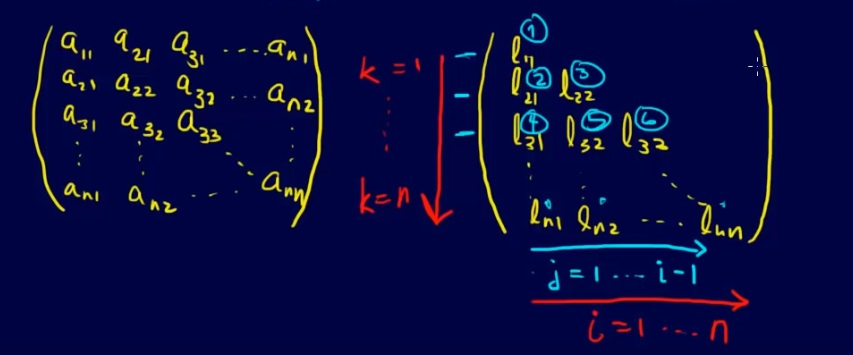
\includegraphics[height=5cm]{cholesky.jpg}\\\\\\
\textbf{double** transpose(double **L, double **LTranspose, int n)}\\
Δέχεται δύο δισδιάστατους τετραγωνικούς πίνακες $\mathbf{L}$ και $\mathbf{LTranspose}$, με μέγεθος n επί n. Επιστρέφει τον πίνακα $\mathbf{LTranpose}$, με την εντολή \texttt{return LTranspose;} Σκοπός της συνάρτησης είναι να παράγει τον ανάστροφο πίνακα του $\mathbf{L}$. Να σημειωθεί ότι, στο συγκεκριμένο πρόγραμμα, ο πίνακας $\mathbf{L}$ είναι κάτω τριγωνικός, άρα ο παραγώμενος πίνακας $\mathbf{L^T}$, ο οποίος ανατίθεται στην μεταβλητή \texttt{LTranspose}, θα είναι άνω τριγωνικός. Δηλαδή, \texttt{LTranspose[j][i] = L[i][j]}. Επίσης, με τις δύο εντολές \texttt{LTranspose[i][j] = 0;} και \texttt{L[j][i] = 0;}, ορίζει τα στοιχεία του $\mathbf{LTranpose}$ κάτω από την κύρια διαγώνιο και τα στοιχεία του $\mathbf{L}$ πάνω από την κύρια διαγώνιο, ως μηδέν.\\\\
\textbf{int main()}\\
Αρχικοποιεί τις μεταβλητές, κάποιες με τη χρήση της \texttt{malloc()}, διαβάζει το μέγεθος \texttt{n} και με τις κατάλληλες συναρτήσεις διαβάζει τον πίνακα $\mathbf{A}$. Στη συνέχεια, καλεί την συνάρτηση \texttt{double* cholesky()} και αναθέτει το αποτέλεσμά της στον πίνακα $\mathbf{L}$. Έπειτα, καλεί την συνάρτηση \texttt{double* transpose()} και αναθέτει το αποτέλεσμά της στον πίνακα $\mathbf{LTranspose}$. Με την κατάλληλη συνάρτηση το τυπώνει στην κονσόλα. Τέλος, καθαρίζει τη μνήμη από παραπάνω χρήσεις της \texttt{malloc()}. Ο κώδικας υπάρχει στον φάκελο \emph{3b}, με όνομα \emph{`main.c`}.\\



\subsection*{Γ' Ερώτημα - Gauss Seidel}  % Adds subsection
Ο κώδικας χωρίστηκε σε πολλές συναρτήσεις για να είναι περισσότερο κατανοητός:\\\\
\textbf{void writeVector(double *x, int n)}\\
	Δέχεται διάνυσμα $\mathbf{x}$, με διάσταση n, και τυπώνει τα στοιχεία του στην κονσόλα.\\\\
\textbf{void copyVector(double *x, double *y, int n)}\\
	Δέχεται δύο διανύσματα $\mathbf{x}$ και $\mathbf{y}$, διάστασης n, και αντιγράφει τα στοχεία του $\mathbf{x}$ στο $\mathbf{y}$, ένα προς ένα.\\\\
\textbf{void initializeA(double **X, int n)}\\
	Δέχεται δισδιάστατο τετραγωνικό πίνακα $\mathbf{X}$, με μέγεθος n επί n, και τον αρχικοποιεί ώστε να είναι ίδιος με αυτόν της εκφώνησης.\\\\
\textbf{void initializeX(double *x, int n)}\\
	Δέχεται διάνυσμα $\mathbf{x}$, διάστασης n, και τον αρχικοποιεί με μηδενικά στοιχεία. Δηλαδή, η πρώτη προσέγγιση των λύσεων, είναι το μηδενικό διάνυσμα.\\\\
\textbf{void initializeB(double *b, int n)}\\
	Δέχεται διάνυσμα $\mathbf{b}$, διάστασης n, και το αρχικοποιεί ώστε να είναι ίδιο με αυτό της εκφώνησης.\\\\
\textbf{double* substract(double *x, double *y, double *z, int n)}\\
	Δέχεται τρία διανύσμα $\mathbf{x}$, $\mathbf{y}$, $\mathbf{z}$ διάστασης n, και επιστρέφει το διάνυσμα $\mathbf{z}$ όπου $\mathbf{z}$ = $\mathbf{x}$ - $\mathbf{y}$.\\\\
\textbf{double calculateInfinityNorm(double *x, int n)}\\
	Δέχεται διάνυσμα $\mathbf{x}$, διάστασης n, υπολογίζει και επιστρέφει την άπειρη νόρμα του.\\\\
\textbf{double* gaussSeidel(double **A, double *x, double *b, double *prevX, int n)}\\
	Δέχεται δισδιάστατο τετραγωνικό πίνακα $\mathbf{A}$, με μέγεθος n επί n, τρία διανύσματα $\mathbf{x}$, $\mathbf{b}$, $\mathbf{prevX}$, διάστασης n. Υπολογίζει με τη μέθοδο Gauss-Seidel ένα διάνυσμα προσέγγισης ρίζας του γραμμικού συστήματος $\mathbf{Α}\mathbf{x}=\mathbf{b}$ με ακρίβεια τεσσάρων δεκαδικών ψηφίων, το αναθέτει στο διάνυσμα $\mathbf{x}$ και το επιστρέφει. Οι τιμές του υπολογίζονται σύμφωνα με τον τύπο:\\
$(x_i)^{(m+1)} = \frac{1}{a_{ii}}( b_i - \sum_{j=1}^{i-1}(a_{ij}{x_j}^{(m+1)}) - \sum_{j=i+1}^{n}({a_{ij}}{x_j}^{(m)}) )$ με $i = 1,..,n$ και $m=1,..$\\\\
\textbf{int main()}\\
Αρχικοποιεί τις μεταβλητές, κάποιες με τη χρήση της \texttt{malloc()}, διαβάζει το μέγεθος \texttt{n} και με τις κατάλληλες συναρτήσεις αρχικοποεί τα $\mathbf{A}$, $\mathbf{x}$ και $\mathbf{b}$. Στη συνέχεια, έχει μια επανάληψη \texttt{do-while} που τερματίζει όταν \texttt{infinityNorm < TOLERANCE} με \texttt{TOLERANCE = 0.00005}. Μέσα στην επανάληψη, υπολογίζεται κάθε προσέγγιση λύσεων του γραμμικού συσήματος, δηλαδή το διάνυσμα $\mathbf{x}$, με τη παραπάνω μέθοδο Gauss Seidel. Έπειτα υπολογίζει το $\mathbf{y}=\mathbf{x_n}-\mathbf{x_{n-1}}$, και τη νόρμα του, ώστε να ελέγξει τη συνθήκη τερματίζει την επανάληψη. Με την κατάλληλη συνάρτηση τυπώνει στην κονσόλα την τελική προσέγγιση $\mathbf{x}$. Τέλος, καθαρίζει τη μνήμη από παραπάνω χρήσεις της \texttt{malloc()}.\\\\
Ο αλγόριθμος εκτελέστηκε για n=10 (σε σχεδόν μηδενικό χρόνο) και για n=10000 (κάτω από δέκα δευτερόλεπτα), και όλες οι λύσεις προσεγγίζουν το 1. Ο κώδικας υπάρχει στον φάκελο \emph{3c}, με όνομα \emph{`main.c`}.\\\\


\section*{Τέταρτη Άσκηση}   % Starts fourth exercise

\subsection*{Α' Ερώτημα - Απόδειξη ότι $\mathbf{G}$ είναι στοχαστικός}  % Adds subsection
Ο τύπος για το κάθε στοιχείο του πίνακα $\mathbf{G}$ είναι ο εξής: $\mathbf{G}_{ij} = \frac{q}{n} + \frac{\mathbf{A}_{ji}(1-q)}{n_j}$.\\ Τα $q,n$ είναι σταθερές, και το $n_j$ αποτελεί το άθροισμα της $j$ γραμμής του πίνακα $\mathbf{A}$, δηλαδή θα ισχύει ότι $n_j = \sum_{i=1}^{n}\mathbf{A}_{ji}$. Σύμφωνα με την εκφώνηση, ο πίνακας $\mathbf{G}$ είναι στοχαστικός, αφού το άθροισμα κάθε στήλης του ισούται με 1. Ας το αποδείξουμε ως εξής:\\
Έστω, ότι $j$ είναι μια οποιαδήποτε στήλη του πίνακα $\mathbf{G}$. Πρέπει να αποδείξουμε ότι άθροισμα αυτής της οποιασδήποτε στήλης, ισούται με 1, δηλαδή $\sum_{i=1}^{n}\mathbf{G}_{ij} = 1$. Ισχύει ότι:\\\\$\sum_{i=1}^{n}\mathbf{G}_{ij} = \sum_{i=1}^{n}(\frac{q}{n} + \frac{\mathbf{A}_{ji}(1-q)}{n_j}) = \sum_{i=1}^{n}(\frac{q}{n}) + \sum_{i=1}^{n}(\frac{\mathbf{A}_{ji}(1-q)}{n_j}) =\\= n\frac{q}{n} + \frac{1-q}{n_j}\sum_{i=1}^{n}(\mathbf{A}_{ji}) = q + \frac{1-q}{n_j}n_j = q + 1 - q = 1$\\\\Άρα, εφόσον για οποιαδήποτε στήλη του $\mathbf{G}$ ισχύει ότι το άθροισμα της ισούται με την μονάδα, τότε ο πίνακας $\mathbf{G}$ είναι στοχαστικός.
\\\\

\subsection*{Β' Ερώτημα - Πίνακας $\mathbf{G}$ και ιδιοδιανύσματα}  % Adds subsection
Αρχικά, για το συγκεκριμένο ερώτημα γράφηκε κώδικας στον οποίο \textbf{δεν χρησιμοποιήθηκε καθόλου κάποιο γλωσσικό μοντέλο για την διευκόλυνση της γραφής του.} Στην αρχή, με τις κατάλληλες συναρτήσεις, υπολογίζει τον πίνακα Α και κατασκευάζει τον πίνακα $\mathbf{G}$ σύμφωνα με τον τύπο $\mathbf{G}_{ij} = \frac{q}{n} + \frac{\mathbf{A}_{ji}(1-q)}{n_j}$. Στη συνέχεια, τον τυπώνει στην οθόνη. Παρατηρούμε ότι ο πίνακας $\mathbf{G}$, είναι πράγματι στοχαστικός, καθώς κάθε άθροισμα στήλης του ισούται με 1 (ή έστω το προσεγγίζει σε πολύ μεγλάλο βαθμό σε περίπτωση που χαθεί κάποιο δεκαδικό ψηφίο).\\\\
$\mathbf{G} = 
\begin{smallmatrix}
0.010 & 0.010 & 0.010 & 0.010 & 0.435 & 0.010 & 0.010 & 0.010 & 0.010 & 0.010 & 0.010 & 0.010 & 0.010 & 0.010 & 0.010 \\
0.435 & 0.010 & 0.293 & 0.010 & 0.010 & 0.010 & 0.010 & 0.010 & 0.010 & 0.010 & 0.010 & 0.010 & 0.010 & 0.010 & 0.010 \\
0.010 & 0.293 & 0.010 & 0.435 & 0.010 & 0.010 & 0.010 & 0.010 & 0.010 & 0.010 & 0.010 & 0.010 & 0.010 & 0.010 & 0.010 \\
0.010 & 0.010 & 0.010 & 0.010 & 0.010 & 0.010 & 0.010 & 0.435 & 0.010 & 0.010 & 0.010 & 0.010 & 0.010 & 0.010 & 0.010 \\
0.010 & 0.293 & 0.010 & 0.010 & 0.010 & 0.010 & 0.010 & 0.010 & 0.293 & 0.010 & 0.010 & 0.010 & 0.010 & 0.010 & 0.010 \\
0.010 & 0.010 & 0.293 & 0.010 & 0.010 & 0.010 & 0.010 & 0.010 & 0.293 & 0.010 & 0.010 & 0.010 & 0.010 & 0.010 & 0.010 \\
0.010 & 0.293 & 0.010 & 0.010 & 0.010 & 0.010 & 0.010 & 0.010 & 0.010 & 0.010 & 0.010 & 0.293 & 0.010 & 0.010 & 0.010 \\
0.010 & 0.010 & 0.293 & 0.010 & 0.010 & 0.010 & 0.010 & 0.010 & 0.010 & 0.010 & 0.010 & 0.293 & 0.010 & 0.010 & 0.010 \\
0.435 & 0.010 & 0.010 & 0.010 & 0.010 & 0.010 & 0.010 & 0.010 & 0.010 & 0.010 & 0.010 & 0.010 & 0.435 & 0.010 & 0.010 \\
0.010 & 0.010 & 0.010 & 0.010 & 0.435 & 0.435 & 0.435 & 0.010 & 0.293 & 0.010 & 0.010 & 0.010 & 0.010 & 0.223 & 0.010 \\
0.010 & 0.010 & 0.010 & 0.010 & 0.010 & 0.435 & 0.435 & 0.435 & 0.010 & 0.010 & 0.010 & 0.293 & 0.010 & 0.223 & 0.010 \\
0.010 & 0.010 & 0.010 & 0.435 & 0.010 & 0.010 & 0.010 & 0.010 & 0.010 & 0.010 & 0.010 & 0.010 & 0.010 & 0.010 & 0.435 \\
0.010 & 0.010 & 0.010 & 0.010 & 0.010 & 0.010 & 0.010 & 0.010 & 0.010 & 0.860 & 0.010 & 0.010 & 0.010 & 0.223 & 0.010 \\
0.010 & 0.010 & 0.010 & 0.010 & 0.010 & 0.010 & 0.010 & 0.010 & 0.010 & 0.010 & 0.010 & 0.010 & 0.435 & 0.010 & 0.435 \\
0.010 & 0.010 & 0.010 & 0.010 & 0.010 & 0.010 & 0.010 & 0.010 & 0.010 & 0.010 & 0.860 & 0.010 & 0.010 & 0.223 & 0.010 \\\\
\end{smallmatrix}
$
	Στη συνέχεια, με τη μέθοδο των δυνάμεων, ο κώδικας υπολογίζει στη συνάρτηση \texttt{void powerMethod(double **G, double *eigenVector, int n)} το διάνυσμα της μέγιστης ιδιοτιμής, η οποία ισούται με την μονάδα γιατί ο πίνακας $\mathbf{G}$ είναι στοχαστικός. Ο επαναληπτικός αλγόριθμος σταματάει όταν ισχύσει\\ \texttt{sub < TOLERANCE}. Η σταθερά \texttt{TOLERANCE} ορίστηκε \texttt{0.00000000005} (δηλαδή ακρίβεια 10 δεκαδικών ψηφίων). Η μεταβλητή \texttt{sub} αντιπροσοπεύει την διαφορά\\ $|b_n[0] - b_{n-1}[0]|$, όπως ορίζει ο αλγόριθμος της μεθόδου των δυνάμεων. Στην αρχή, αρχικοποιείται ως πρώτη προσέγγιση του ιδιοδιανύσματος, ένα τυχαίο διάνυσμα-στήλη του πίνακα $\mathbf{G}$. Διάλεξα το πρώτο, δηλαδή το \texttt{G[0]}. Μέσα στην επανάληψη \texttt{do-while}, υπολογίζεται, αρχικά, το νέο διάνυσμα προσέγγισης του ιδιοδιανύσματος με τον γνωστό τύπο: $b_{n+1} = \mathbf{G}b_n$. Για να γίνει αυτός ο πολλαπλασιασμός, χρησιμοποιείται η βοηθητική συνάρτηση \texttt{void* multiply(double **P, double *b, double *c, int n)}, που εξυπηρετεί ακριβώς αυτόν τον σκοπό. Στη συνέχεια, κανονικοποιώ το διάνυσμα (και το αναθέτω σε διαφορετική μεταβλητή), έτσι όπως ορίζει η εκφώνηση, δηλαδή με τέτοιον τρόπο ώστε το άθροισμα των τιμών του να ισούται με την μονάδα. Επομένως, το πολλαπλασιάζω με το $\frac{1}{\texttt{factor}}$, όπου το \texttt{factor} ισούται με το άθροισμα των τιμών του. Ο πολλαπλασιασμός με το $\frac{1}{\texttt{factor}}$ γίνεται με τη βοήθεια της συνάρτησης \\ \texttt{double* multiply2(double l, double *b, double* c, int n)}, η οποία εξυπηρετεί αυτόν τον σκοπό. Η εύρεση του \texttt{factor}, δηλαδή του αθροίσματος των τιμών του διανύσματος, γίνεται με τη χρήση της βοηθητικής συνάρτησης \texttt{double findFactor(double* x, int n)}. Έπειτα, υπολογίζεται το \texttt{sub} με τον τρόπο που αναφέρθηκε παραπάνω. Στη συνέχεια, το νέο διάνυσμα ορίζεται ως το παλίο, με τη χρήση της βοηθητικής συνάρτησης \texttt{void copyVector(double *x, double *y, int n)}, ώστε να χρησιμοποιηθεί στην νέα επανάληψη για να βρεθεί μια καινούργια προσσέγιση. Τέλος, ελέγχεται η συνθήκη τερματισμού, η οποία αναλύθηκε παραπάνω. Στην \texttt{int main()}, γίνονται οι κατάλληλες αρχικοποιήσεις και κλήσεις των συναρτήσεων που αναφέρθηκαν παραπάνω, ώστε να υπολογιστεί και να εμφανιστεί το αποτέλσμα στην οθόνη. Η τελική προσέγγιση, είναι πολύ κοντινή στο διάνυσμα $\textbf{b}$ που δίνεται στην εκφώνηση:\\\\
$\mathbf{b_n} = [0.0268246, 0.0298611, 0.0298611, 0.0268246, 0.0395872, 0.0395872, 0.0395872,\\ 0.0395872, 0.0745644, 0.1063200, 0.1063200, 0.0745644, 0.1250916, 0.1163279,  0.1250916]$\\\\
Ο κώδικας υπάρχει στον φάκελο \emph{4b}, με όνομα \emph{`main.c`}.
\\\\

\subsection*{Γ' Ερώτημα - Τροποποίηση συνδέσεων}  % Adds subsection
Έστω ότι το διάνυσμα:\\\\
$\mathbf{b_n} = [0.0268246, 0.0298611, 0.0298611, 0.0268246, 0.0395872, 0.0395872, 0.0395872,\\ 0.0395872, 0.0745644, 0.1063200, 0.1063200, 0.0745644, 0.1250916, 0.1163279,  0.1250916]$\\\\ αντιπροσωπεύει τις τάξεις των σελιδών. Παρατηρούμε ότι η σελίδα 2 και 3 (με τάξεις \texttt{b[1]} και \texttt{b[2]} αντίστοιχα), έχουν πολύ κοντινές τάξεις. Στο συγκεκριμένο διάνυσμα φαίνονται ίδιες, αλλά υπάρχει μεγάλη πιθανότητα να είναι λίγο διαφορετικές, λόγω απώλειας δεκαδικών ψηφίων. Σκοπός του ερωτήματος είναι η βελτίωση της σημαντικότητας της 2ης σελίδας, ώστε να ξεπεράσει τον κύριο ανταγωνιστή της, την 3η. Λόγω της εκφώνησης, τέθηκαν περιορισμοί 1 αφαίρεσης και 4 προσθηκών στις συνδέσεις των σελιδών, δηλαδή στον πίνακα $\mathbf{Α}$. Αυτό θα έχει αλλαγή στον πίνακα $\mathbf{G}$, άρα και στο διάνυσμα με τη μέγιστη ιδιοτιμή, δηλαδή στο διάνυσμα τάξης των σελίδων. Για να βελτιωθεί η 2η σελίδα σε σχέση με την 3η, αφαιρέθηκε η σχέση που δείχνει από την 2η σελίδα στην 3η, και προστέθηκαν σχέσεις που προέρχονται από σελίδες με υψηλές τάξεις (11, 13, 14, 15) και δείχνουν στην 2. Δηλαδή ο δοσμένος πίνακας $\mathbf{Α}$ δέχθηκε τις εξής αλλαγές:\\\\
A[1][2] = 0, αφαιρέθηκε η σχέση που δείχνει από την 2η σελίδα στην 3η.\\
A[10][1] = 1, προστέθηκε η σχέση που δείχνει από την 11η σελίδα στην 2η.\\
A[12][1] = 1, προστέθηκε η σχέση που δείχνει από την 13η σελίδα στην 2η.\\
A[13][1] = 1, προστέθηκε η σχέση που δείχνει από την 14η σελίδα στην 2η.\\
A[14][1] = 1, προστέθηκε η σχέση που δείχνει από την 15η σελίδα στην 2η.\\
Έτσι, εκτελέστηκε το πρόγραμμα του Β' Ερωτήματος, με τις προηγούμενες αλλαγές. Το νέο διάνυσμα τάξεων εμφανίστηκε ως εξής:\\\\
$\mathbf{b'_n} = 0.0464889, 0.1350706, 0.0188263, 0.0207677, 0.0858563, 0.0337854, 0.0774065,\\ 0.0253356, 0.0651221, 0.1227091, 0.0885381, 0.0352996, 0.1248151, 0.0618376, 0.0581411]$\\\\
Παρατηρούμε ότι η τάξη της 2ης σελίδας βελτιώθηκε κατά πολύ (περίπου 352 τοις εκατό). Παρ'όλα αυτά, το διάνυσμα $\mathbf{b'_n}$ είναι κανονικοποιημένο ώστε το άθροισμα των τιμών του να είναι πάντα 1. Οπότε, είναι αυτονόητο, όταν αυξηθεί ένα στοιχείο (δηλαδή μια τάξη), να μειωθεί κάποιο/κάποια άλλα, ώστε να διατηρηθεί αυτή η ιδιότητα. Ας παρατηρήσουμε τις αλλαγές μεταξύ του $\mathbf{b_n}$ (του προηγούμενο υποερωτήματος) και του $\mathbf{b'_n}$ (του συγκεκριμένου υποερωτήματος):\\\\
$\mathbf{b_n} = [0.0268246, 0.0298611, 0.0298611, 0.0268246, 0.0395872, 0.0395872, 0.0395872,\\ 0.0395872, 0.0745644, 0.1063200, 0.1063200, 0.0745644, 0.1250916, 0.1163279,  0.1250916]$\\\\
$\mathbf{b'_n} = 0.0464889, 0.1350706, 0.0188263, 0.0207677, 0.0858563, 0.0337854, 0.0774065,\\ 0.0253356, 0.0651221, 0.1227091, 0.0885381, 0.0352996, 0.1248151, 0.0618376, 0.0581411]$\\\\
Βλέπουμε λοιπόν ότι παρόλο που οι αλλαγές εμπλέκουν \textbf{άμεσα} μόνο τις σελίδες 2,3,11,13,14,15, άλλαξε η σημαντικότητα όλων των σελίδων. Αυτό συμβαίνει επειδή, έμμεσα, όλες σελίδες συνδέονται μεταξύ τους, μέσω κάποιας-κάποιων σελίδων που μεσολαβούν ανάμεσά τους. Επομένως η συγκεκριμένη αλλαγή, που περιέχει μόνο 15 σελίδες, δείχνει πόσο πολύπλοκο και πολυσύνθετο είναι ό,τι κρύβεται πίσω από τη σημαντικότητα των σελιδών στις σημερινές μηχανές αναζήτησης σελίδες (που περιέχουν εκατομμύρια σελίδες). Ο κώδικας υπάρχει στον φάκελο \emph{4c}, με όνομα \emph{`main.c`}.
\\\\

\subsection*{Δ' Ερώτημα - Πιθανότητα μεταπήδησης}  % Adds subsection
Υπενθυμίζουμε ότι το διάνυσμα με τις τάξεις των σελιδών, όπως παράχθηκε από το πρόγραμμα του Β' Ερωτήματος, είναι το εξής:\\\\
$\mathbf{b0_n} = [0.0268246, 0.0298611, 0.0298611, 0.0268246, 0.0395872, 0.0395872, 0.0395872,\\ 0.0395872, 0.0745644, 0.1063200, 0.1063200, 0.0745644, 0.1250916, 0.1163279,  0.1250916]$\\\\
Ας αλλάξουμε την πιθανότητα μεταπήδησης \texttt{q}, από \texttt{0.15} σε \texttt{α) 0.02} και \texttt{β) 0.6}.\\\\
Για \texttt{q = 0.02}, τρέχοντας το ίδιο πρόγραμμα, παρήχθηκε το εξής διάνυσμα:\\\\
$\mathbf{b1_n} = [0.0171063, 0.0144289, 0.0144289, 0.0171063, 0.0321898, 0.0321898, 0.0321898,\\ 0.0321898, 0.0800297, 0.1095760, 0.1095760, 0.0800297, 0.1434985, 0.1419619, 0.1434985]$\\\\
Βλέπουμε ότι, εφόσον μειώνουμε την πιθανότητα μεταπήδησης, τότε η σημαντικότητα της σελίδας θα εξαρτηθεί περισσότερο από τον παράγοντα της συνδεσιμότητας. Δηλαδή, αν η τάξη μιας σελίδας βασιζόταν περισσότερο στην πιθανότητα μεταπήδησης, δηλαδή στο γεγονός να βρεθεί τυχαία ο χρήστης εκεί, χωρίς να μετακινηθεί στον σύνδεσμό της από κάποια άλλη σελίδα, τότε είναι φυσικό αυτή η τάξη να μειωθεί. Για παράδειγμα, η σελίδα 1, που βασίζεται κυρίως στην πιθανότητα μεταπήδησης, καθώς σύμφωνα με το γράφο υπάρχουν λίγες διαδρομές που καταλήγουν σε αυτήν σε σχέση με τις υπόλοιπες σελίδες, υπέστη μείωση της τάξης της. Συγκεκριμένα, από 0.0268246 μειώθηκε σε 0.0171063 (περίπου 36 τοις εκατό μείωση). Αναλόγως, αν η τάξη μιας σελίδας βασιζόταν περισσότερο στη συνδεσιμότητα, δηλαδή να καταλήγουν πολλές διαδρομές του γράφου σε αυτή και ο χρήστης να μπορεί να βρεθεί αυτή μέσω συνδέσμων και όχι τυχαία, τότε είναι φυσικό αυτή η τάξη να αυξηθεί. Για παράδειγμα, η σελίδα 15, που βασίζεται κυρίως στη συνδεσιμότητα, καθώς πολλές διαδρομές του γράφου καταλήγουν σε αυτή σε σχέση με άλλες σελίδες, υπέστη αύξηση της τάξης της. Συγκεκριμένα, από 0.1250916 αυξήθηκε σε 0.1434985 (περίπου 15 τοις εκατό αύξηση).\\\\
Για \texttt{q = 0.6}, τρέχοντας το ίδιο πρόγραμμα, παράχθηκε το εξής διάνυσμα:\\\\
$\mathbf{b2_n} = [0.0513321, 0.0579997, 0.0579997, 0.0513321, 0.0566606, 0.0566606, 0.0566606,\\ 0.0566606,  0.0669549,  0.0902614, 0.0902614, 0.0669549, 0.0834422, 0.0733769, 0.0834422]$\\\\
Βλέπουμε ότι, εφόσον αυξάνουμε την πιθανότητα μεταπήδησης, τότε η σημαντικότητα της σελίδας θα εξαρτηθεί λιγότερο από τον παράγοντα της συνδεσιμότητας. Δηλαδή, αν η τάξη μιας σελίδας βασιζόταν περισσότερο στην πιθανότητα μεταπήδησης, δηλαδή στο γεγονός να βρεθεί τυχαία ο χρήστης εκεί, χωρίς να μετακινηθεί στον σύνδεσμό της από κάποια άλλη σελίδα, τότε είναι φυσικό αυτή η τάξη να αυξηθεί. Για παράδειγμα, η σελίδα 1, που βασίζεται κυρίως στην πιθανότητα μεταπήδησης, καθώς σύμφωνα με το γράφο υπάρχουν λίγες διαδρομές που καταλήγουν σε αυτήν σε σχέση με τις υπόλοιπες σελίδες, υπέστη αύξηση της τάξης της. Συγκεκριμένα, από 0.0268246 αυξήθηκε σε 0.0513321 (περίπου 91 τοις εκατό αύξηση). Αναλόγως, αν η τάξη μιας σελίδας βασιζόταν περισσότερο στη συνδεσιμότητα, δηλαδή να καταλήγουν πολλές διαδρομές του γράφου σε αυτή και ο χρήστης να μπορεί να βρεθεί αυτή μέσω συνδέσμων και όχι τυχαία, τότε είναι φυσικό αυτή η τάξη να μειωθεί. Για παράδειγμα, η σελίδα 15, που βασίζεται κυρίως στη συνδεσιμότητα, καθώς πολλές διαδρομές του γράφου καταλήγουν σε αυτή σε σχέση με άλλες σελίδες, υπέστη μείωση της τάξης της. Συγκεκριμένα, από 0.1250916 μειώθηκε σε 0.0834422 (περίπου 33 τοις εκατό μείωση).\\\\
Γενικά, η πιθανότητα μετάβασης εκφράζει το ποσοστό πιθανότητας που ένας χρήστης θα μετακινηθεί από μια σελίδα σε μια άλλη χωρίς να ακολουθήσει συνδέσμους. Αυτός ο παράγοντας εισάγει ένα επίπεδο τυχαιότητας στο μοντέλο, αποτρέποντας τον αλγόριθμο από το να γίνει υπερβολικά ευαίσθητος σε συγκεκριμένες παραμέτρους. Αυτό έχει ως αποτέλεσμα μια πιο ισορροπημένη αξιολόγηση της σημασίας μιας σελίδας, λαμβάνοντας υπόψη τη συνδεσιμότητά της καθώς και την πιθανότητα τυχαίας μετάβασης. Συνεπώς, η πιθανότητα μετάβασης βοηθάει τον αλγόριθμο στο να παρέχει μια πιο ρεαλιστική αναπαράσταση της σημασίας των ιστοσελίδων, αντιμετωπίζοντας το διαδίκτυο ως ένα δυναμικό και πολυπλοκό σύστημα που περιλαμβάνει τυχαίες μεταβάσεις μεταξύ των σελίδων.\\\\ Οι κώδικες υπάρχουν στον φάκελο \emph{4d}, με ονόματα \emph{`main1.c`} και \emph{`main2.c`} αντίστοιχα.

\subsection*{Ε' Ερώτημα - Αλλαγή πίνακα γειτνίασης}  % Adds subsection
Υπενθυμίζουμε ότι το διάνυσμα με τις τάξεις των σελιδών, όπως παράχθηκε από το πρόγραμμα του Β' Ερωτήματος, είναι το εξής:\\\\
$\mathbf{b_n} = [0.0268246, 0.0298611, 0.0298611, 0.0268246, 0.0395872, 0.0395872, 0.0395872,\\ 0.0395872, 0.0745644, 0.1063200, 0.1063200, 0.0745644, 0.1250916, 0.1163279,  0.1250916]$\\\\
Σε αυτό το ερώτημα, έγινε η εξής αλλαγή στον πίνακα γειτνίασης: \texttt{A[7][10] = 3} και \texttt{A[11][10] = 3}, ενώ αντί για 3 είχαν 1. Δηλαδή, βελτιώθηκαν οι σχέσεις που δείχνουν από τις σελίδες 8 και 12 στην σελίδα 11. Έτσι, εκτελέστηκε το πρόγραμμα του Β' Ερωτήματος με τις εξής αλλαγές. Το νέο διάνυσμα τάξεων είναι το εξής:\\\\
$\mathbf{b'_n} = [0.0265505, 0.0283717, 0.0250156, 0.0164163, 0.0389424, 0.0379915, 0.0311454,\\ 0.0301945, 0.0737779, 0.1028933, 0.1240084, 0.0770987, 0.1235151, 0.1226157, 0.1414629]$\\\\
Όπως βλέπουμε επηρεάστηκαν όλες οι τάξεις, και πράγματι η σελίδα 11 βελτίωσε την τάξη (16 τοις εκατό αύξηση) της σε σχέση με τον ανταγωνιστή της, την σελίδα 10 (3 τοις εκατό μείωση). Η διαφορά των δυό νέων τάξεων, υπέρ της 11, από 0 έγινε 0.0211151. Ας αναλύσουμε τον λόγο που αυξήθηκε η σελίδα 11. Αλλάζοντας τον πίνακα γειτνίασης $\mathbf{A}$, αλλάζουμε τον πίνακα Google $\mathbf{G}$, καθώς δίνεται από τον τύπο: $\mathbf{G}_{ij} = \frac{q}{n} + \frac{\mathbf{A}_{ji}(1-q)}{n_j}$, και επομένως τη σημαντικότητα της κάθε σελίδας. Δηλαδή, αν η τιμή 3 αντί για 1 προστεθεί στο \texttt{A[j][i]}, τότε η σχέση αυτή θα έχει μεγαλύτερο βάρος, διότι ουσιαστικά πολλαπλασιάζεται με $\frac{(1-Q)}{sumRow(A[j], n)}.$ Άρα, η τιμή 3 θα δίνει μεγαλύτερο βάρος στις σχέσεις που τη χρησιμοποιούν σε σχέση με την τιμή 1. Στη συνέχεια, το άθροισμα της γραμμής 10 (δηλαδή της σελίδας 11) στον πίνακα $\mathbf{G}$, αυξήθηκε. Επίσης, και άλλες σελίδες που η τάξη τους επηρεάζονται έμμεσα από τις σχέσεις της 8 και 12 με την 11, υπέστησαν αύξηση τάξης, εφόσον αυτές οι σχέσεις ενισχύθηκαν. Ενώ, άλλες σελίδες που επηρεαζόταν λιγότερο ή καθόλου, υπέστησαν μείωση τάξης, όπως η σελίδα 10. Συνεπώς, στη συγκεκριμένη περίπτωση, η στρατηγική δούλεψε και οι παραπάνω λόγοι είναι αυτοί που οδήγησαν στην μεταβολή της τάξης της σελίδας 11, αλλά και όλων των υπολοίπων. Αυτό το ερώτημα, όπως και το Γ', δείχνει πόσο πολύπλοκο και πολυσύνθετο είναι ό,τι κρύβεται πίσω από τη σημαντικότητα των σε λιδών στις σημερινές μηχανές αναζήτησης σελίδες, καθώς όλα συνδέονται. Ο κώδικας υπάρχει στον φάκελο \emph{4e}, με όνομα \emph{`main.c`}.

\subsection*{ΣΤ' Ερώτημα - Διαγραφής σελίδας 10}  % Adds subsection
Υπενθυμίζουμε ότι το διάνυσμα με τις τάξεις των σελιδών, όπως παράχθηκε από το πρόγραμμα του Β' Ερωτήματος, είναι το εξής:\\\\
$\mathbf{b_n} = [0.0268246, 0.0298611, 0.0298611, 0.0268246, 0.0395872, 0.0395872, 0.0395872,\\ 0.0395872, 0.0745644, 0.1063200, 0.1063200, 0.0745644, 0.1250916, 0.1163279,  0.1250916]$\\\\
Σε αυτό το ερώτημα, άλλαξε ο πίνακας γειτνίασης: \texttt{A}, καθώς αφαιρέθηκε η σελίδα 10. Η αλλαγή του πίνακα \texttt{A} επέφερε αλλαγές στον πίνακα \texttt{G} και επομένως στο διάνυσμα τάξεων. Εκτελέστηκε παρόμοιο πρόγραμμα του Β' Ερωτήματος με τις παραπάνω αλλαγές. Το νέο διάνυσμα τάξεων που παράχθηκε είναι το εξής:\\\\
$\mathbf{b'_n} = [0.0470950, 0.0409114, 0.0359356, 0.0320700, 0.0428008, 0.0413910, 0.0516587,\\ 0.0502489, 0.0482235, 0.1709627, 0.1035981,  0.0411619, 0.1074622, 0.1864802]$\\\\
Ας δούμε τις αλλαγές στις τάξεις:\\
Σελίδες που υπέστησαν άυξηση στην τάξη τους: 1, 2, 3, 4, 5, 6, 7, 8, 11, 12, 15\\
Σελίδες που υπέστησαν άυξηση στην τάξη τους: 9, 13, 14\\\\
Η τάξη της κάθε σελίδας μειώθηκε ή αυξήθηκε, ανάλογα με το πόσο στενά συνδεόταν με τη διαγραφόμενη σελίδα 10. Για παράδειγμα, ας αναλύσουμε τις μειώσεις τάξεων. Η σελίδα 10 έδειχνε άμεσα στην 13, και γι'αυτό η 13 υπέστη μείωση τάξης. Η σελίδα 13, που την έδειχνε η 10, έδειχνε αντίστοιχα στην 14 και στην 9, οι οποίες κι αυτές δέχτηκαν μείωση τάξης. Αξίζει να σημειωθεί ότι η σελίδα 13, που συνδεόταν \textbf{άμεσα} με την σελίδα 10, υπέστη την μεγαλύτερη μείωση τάξης (67 τοις εκατό μείωση). Δηλαδή, η μόνη σελίδα που έδειχνε άμεσα η 10, ήταν η 13. Αυτό το ερώτημα, όπως το Γ' και το Ε', δείχνει πόσο πολύπλοκο και πολυσύνθετο είναι ό,τι κρύβεται πίσω από τη σημαντικότητα των σε λιδών στις σημερινές μηχανές αναζήτησης σελίδες, καθώς όλα συνδέονται. Ο κώδικας υπάρχει στον φάκελο \emph{4st}, με όνομα \emph{`main.c`}.\\\\\\
\end{document}   % Mark the ending of the main content of the document.